\documentclass[letterpaper,journal]{IEEEtran}
\PassOptionsToPackage{hyphens}{url}
\usepackage[T1]{fontenc}
\usepackage{mathptmx}
\renewcommand{\ttdefault}{cmtt}
\usepackage{graphicx,booktabs,amsmath,amssymb,url,multirow,array,enumitem,etoolbox,microtype}
\usepackage[hidelinks]{hyperref}
\Urlmuskip=0mu plus 1mu\relax
\setlist[itemize]{nosep,leftmargin=1.25em,topsep=2pt}
\setlist[enumerate]{nosep,leftmargin=1.45em,topsep=2pt}
\linespread{0.932}
\renewcommand{\arraystretch}{1.0}
\setlength{\textfloatsep}{8pt plus 2pt minus 2pt}
\setlength{\dbltextfloatsep}{8pt plus 2pt minus 2pt}
\setlength{\floatsep}{6pt plus 2pt minus 2pt}
\setlength{\dblfloatsep}{6pt plus 2pt minus 2pt}
\setlength{\abovecaptionskip}{3.5pt}
\AtBeginDocument{%
  \setlength{\abovedisplayskip}{5pt plus 2pt minus 2pt}%
  \setlength{\belowdisplayskip}{5pt plus 2pt minus 2pt}%
}
\newcommand{\cb}{\texttt{cost\_bid}}
\newcommand{\gb}{\texttt{group\_bid}}

\begin{document}
\bstctlcite{IEEEexample:BSTcontrol}

\title{Who Backs Into the Bay? Benchmarking Information, Incentives, and Sim-to-3D Robustness in Narrow-Corridor Robot Negotiation}

\author{Roshan George, Martin Glavin, Edward Jones, and Brian Deegan%
\thanks{All authors are with the Connaught Automotive Research (CAR) group and the Ryan Institute, University of Galway, Ireland (e-mail: brian.deegan@universityofgalway.ie).}%
\thanks{Manuscript draft prepared for journal submission.}}

\maketitle

\begin{abstract}
When two autonomous mobile robots (AMRs) meet head-on in a corridor too narrow for side-by-side passage, one robot must reverse into a discrete pull-in bay or out into an end room. Resolving such conflicts without a central fleet scheduler requires coupling a discrete negotiation decision---who yields, and into which refuge---with continuous execution under asymmetric forward/reverse kinematics, lossy wireless channels, and onboard perception. We present an open dual-simulator benchmark in which an identical 20\,Hz agent state machine executes both in a fast 2D unicycle simulator (over 50,000 Monte Carlo episodes across 18 factorial studies) and in ROS~2 Jazzy / Gazebo Harmonic with 3D TurtleBot3 Waffles (496 seed-paired runs). Using a hindsight best-forced-yielder reference, we evaluate non-communicating reactive backoff, first-come corridor reservation, fixed priority, lexicographic rulebooks, kinematic cost bidding, convoy group bidding, a Clarke-pivot (VCG) mechanism, and a tabular contextual bandit across four research questions spanning information fidelity, strategic incentives, communication/map resilience, and multi-robot sim-to-3D transfer. Without communication, reactive backoff deadlocks in 6.2\% of single-bay encounters and inflates delay by at least $3.6\times$, whereas every negotiating policy achieves 100\% corridor completion. Under matched kinematics, cost bidding selects the optimal yielder in 100\% of symmetric single- and two-bay encounters and limits urgency-weighted excess delay on heterogeneous robots to $0.04\pm0.02$\,s (vs.\ $27.1\pm2.6$\,s for fixed priority and $18.8\pm0.9$\,s for zone reservation), but loses its advantage over a noise-free closest-refuge rulebook once multiplicative bid error reaches $\sigma=0.5$. Clarke-pivot externality payments eliminate unilateral scaled-misreport gains ($0.00$\,s predicted, $\le 0.02$\,s realized) at the price of a $9.3$--$10.5$\,s/encounter budget surplus and joint-shading vulnerability, while a scalar cumulative-delay credit ($\lambda=0.25$) raises repeated-encounter Jain fairness to $0.997$ for $8.1\%$ extra delay. Across 90--99\% packet loss and partial maps, periodic snapshot broadcast with piggybacked bay lists sustains zero collisions, and 96.8\% (393/406) of Gazebo negotiating runs reproduce 2D yielder choices while exposing concrete sim-to-3D boundaries in lidar peer-cluster latency and three-robot junction timing.
\end{abstract}

\begin{IEEEkeywords}
Autonomous mobile robots, multi-robot coordination, narrow-corridor negotiation, deadlock resolution, mechanism design, ROS~2, Gazebo benchmarking.
\end{IEEEkeywords}

\section{Introduction}
\IEEEPARstart{I}{ntralogistics} warehouses, hospital service wings, semiconductor cleanrooms, and brownfield industrial hallways routinely constrain autonomous mobile robots (AMRs) to single-lane passages where two vehicles cannot pass abreast~\cite{fragapane2021planning,xiao2022barn}. When two differential-drive robots meet head-on in such an aisle, slowing down or swerving laterally is physically insufficient: at least one robot must reverse---typically at a lower speed limit and under degraded rear sensing---into an intermediate pull-in bay or all the way out of the corridor.

Existing multi-robot navigation paradigms sit at two extremes on this problem. Decentralized local collision-avoidance controllers based on velocity obstacles (RVO/ORCA)~\cite{vandenberg2011orca} or control barrier functions (CBFs)~\cite{wang2017safety,grover2023before} require no inter-robot messaging, but reliably fall into symmetric deadlocks in narrow head-on configurations~\cite{grover2023before,dergachev2021distributed,zheng2023deadlock,chandra2025deadlock}. Conversely, centralized multi-agent path finding (MAPF)~\cite{sharon2015cbs,stern2019mapf,okumura2022pibt}, zone-control locks~\cite{fanti2002event}, and industrial fleet managers such as Open-RMF~\cite{openrmf} and VDA~5050~\cite{vda5050} prevent conflicts globally, yet presuppose common map ownership, reliable infrastructure connectivity, and a single coordinating authority---assumptions violated in ad-hoc deployments, radio-shadowed aisles, or multi-vendor facilities~\cite{gautier2022negotiated,gielis2022critical}.

Between reactive avoidance and central scheduling lies \emph{decentralized peer-to-peer negotiation}: encountering robots exchange compact messages over a local broadcast channel and agree on who yields and into which refuge. Over three decades, researchers have proposed fixed social laws and traffic rulebooks~\cite{kato1992coordinating,shoham1995social}, market auctions~\cite{gerkey2002sold,gautier2022negotiated}, incentive-compatible mechanisms and karma economies~\cite{clarke1971multipart,censi2019karma,elokda2024karma}, reinforcement-learned give-way policies~\cite{bettini2022vmas,bettini2023heterogeneous,park2023hallucination}, and recently language-model negotiators~\cite{marlin2024,gamechat2025,garg2024llm}. Despite this breadth, three persistent gaps prevent practitioners from knowing which mechanism to deploy~\cite{chandra2026social,francis2025principles}:
\begin{enumerate}
\item \emph{No shared refuge-and-reversing benchmark:} Prior evaluations test isolated policy families on incompatible point-mass or intersection abstractions that omit nonholonomic turn-and-park maneuvers, asymmetric reverse speeds, and discrete bay placement.
\item \emph{Siloed assumptions on information, incentives, and channels:} Rulebooks assume cooperative agents; auctions assume accurate, truthful cost estimates; mechanism-design studies assume lossless single-shot games; and communication-tolerant protocols rarely quantify excess delay against a per-encounter hindsight reference.
\item \emph{Unverified 2D-to-3D transfer:} Fast 2D kinematic simulators enable large statistical sweeps, yet rarely test whether yield decisions, excess delays, and sensor-gated map-sharing rules survive 3D rigid-body physics, lidar wall-filtering, and asynchronous ROS~2 middleware timing.
\end{enumerate}

Note that we take the symmetric deadlock of continuous reciprocal avoidance (ORCA/RVO/CBF) from the established literature~\cite{grover2023before,dergachev2021distributed,chandra2025deadlock}; our benchmark models a centerline-tracking corridor controller with discrete refuges rather than implementing ORCA or CBF directly. Within this setting, we organize our investigation around two system layers---the \emph{decision mechanism layer} and the \emph{distributed execution and embodiment layer}---and address four research questions:
\begin{itemize}
\item \textbf{RQ1 (Information, Noise \& Generalization):} How much excess delay is saved across zero-comms backoff, corridor reservation, rulebooks, tabular lookup, and kinematic cost bidding---and at what bid error $\sigma$ do rules catch up?
\item \textbf{RQ2 (Strategic Incentives \& Fairness):} How gameable are unpriced and naive-transfer bids, what are the deployment trade-offs of Clarke-pivot (VCG) payments, and how cheaply does scalar delay credit achieve long-run fairness?
\item \textbf{RQ3 (Channel Stress \& Map Uncertainty):} How does a periodic \texttt{STATE}/\texttt{BID} protocol survive 99\% packet loss, which safeguards actually prevent collisions, and how should robots handle mismatched, blocked, or explored maps?
\item \textbf{RQ4 (Multi-Robot Topologies \& 3D Transfer):} How do policies extend to 2-vs.-1 convoys and three-robot T-junctions, and where do 2D conclusions transfer vs.\ break in 3D ROS~2 / Gazebo Harmonic?
\end{itemize}

To answer RQ1--RQ4, this paper contributes:
\begin{enumerate}
\item \textbf{Open Dual-Host Benchmark \& Dataset:} A modular Python/ROS~2 benchmark\footnote{Code, Dockerized ROS~2/Gazebo worlds, study runners, and per-episode datasets: \url{[ANONYMIZED-URL]}.} % TODO: insert archival repository URL/DOI prior to publication
driving the exact same 20\,Hz \texttt{Agent} state machine in \texttt{sim2d} ($>50{,}000$ episodes across 18 studies) and ROS~2 Jazzy / Gazebo Harmonic with TurtleBot3 Waffles (496 seed-paired runs) across six narrow-corridor topologies (Fig.~\ref{fig:scen}).
\item \textbf{Decision-Layer Characterization (RQ1--RQ2):} Paired hindsight-reference evaluation across reactive, reservation, rulebook, bandit, cost-bidding, and Clarke-pivot policies spanning geometry, robot asymmetry, log-normal bid noise ($\sigma\in[0,1]$), 28 misreport profiles, and 20-encounter fairness sequences.
\item \textbf{Protocol Ablation \& Map-Resilience Primitives (RQ3):} A 5,760-episode $2^3$ safeguard ablation at 90--99\% packet loss and 2--8\,s latency showing zero collisions across all arms while revealing that \texttt{commit} adds 3--4\,s delay without deadlock reduction, alongside zero-overhead recovery from map asymmetry via \texttt{BID}-piggybacked bay sets.
\item \textbf{Multi-Robot Extensions \& 496-Run Gazebo Audit (RQ4):} Follower \texttt{make\_room}, side-level \gb, and upstream T-junction \texttt{goal\_wait} primitives, diagnosis of serial convoy yield underpricing, and proof of $96.8\%$ Gazebo yielder agreement ($\le 1.0$\,s corridor excess-delay gap) alongside concrete lidar-clustering and junction-timing transfer boundaries.
\end{enumerate}

The remainder of this paper reviews related work (Sec.~\ref{sec:rel}), formulates the physical encounter and protocol architecture (Sec.~\ref{sec:bench}), defines the policy families and mechanism equations (Sec.~\ref{sec:pol}), details the experimental design and statistical conventions (Sec.~\ref{sec:exp}), presents empirical findings for RQ1--RQ4 (Secs.~\ref{sec:rq1}--\ref{sec:rq4}), synthesizes practitioner guidelines and limitations (Sec.~\ref{sec:disc}), and concludes (Sec.~\ref{sec:conc}).

\section{Related Work}\label{sec:rel}

\subsection{Deadlock in Symmetric and Constrained Navigation}
Local reactive planners such as the Dynamic Window Approach~\cite{fox1997dwa}, Velocity Obstacles~\cite{fiorini1998motion}, RVO/ORCA~\cite{vandenberg2011orca}, and decentralized CBFs~\cite{wang2017safety} achieve scalable collision avoidance in open spaces, yet stall in symmetric head-on bottlenecks where geometric velocity cones or barrier gradients cancel~\cite{grover2023before}. Grover et al.~\cite{grover2023before} formally characterize the equilibrium sets of CBF deadlocks; Zheng and Li~\cite{zheng2023deadlock} perturb nonholonomic controls to escape symmetric stalls; Dergachev and Yakovlev~\cite{dergachev2021distributed} switch stalled ORCA clusters to local MAPF; and Chandra et al.~\cite{chandra2025deadlock,chandra2026social} cast doorway and hallway encounters as ``social mini-games'' resolved via discrete-time CBFs. However, these methods resolve right-of-way where robots can pass after speed modulation or minor lateral shifts. In a single-lane aisle narrower than two robot bodies, liveness requires one robot to select a discrete pull-in bay behind it, reverse into that bay, park clear of the swept lane, and wait until the oncoming stream clears.

\subsection{Centralized Traffic Management, Zone Control, and MAPF}
In structured warehouses, multi-robot coordination is predominantly centralized~\cite{fragapane2021planning}. Classical AGV zone control partitions aisles into mutually exclusive blocks governed by Petri nets or geometric locks~\cite{fanti2002event}, a paradigm directly represented by our first-come \texttt{reservation} baseline. Graph-based MAPF solvers---including CBS~\cite{sharon2015cbs}, PIBT~\cite{okumura2022pibt}, LaCAM~\cite{okumura2023lacam}, safe-interval path planning (SIPP)~\cite{phillips2011sipp}, and narrow-corridor extensions~\cite{experience2024narrow,macga2025}---treat pull-in bays as graph vertices, while kinodynamic planners~\cite{wen2022clmapf,dbecbs2025} and industrial traffic frameworks such as Open-RMF~\cite{openrmf}, VDA~5050~\cite{vda5050}, and hierarchical zone managers~\cite{hiertraffic2023} arbitrate schedules centrally. Precedence-preserving execution protocols~\cite{cap2016provably,mannucci2019provably} further maintain safety under timing delays or unreliable links once a central priority graph is fixed. Unlike those architectures, we study fully decentralized encounter resolution without pre-computed joint schedules, and explicitly penalize the slower reverse kinematics ($0.15$ vs.\ $0.26$\,m/s) that symmetric graph edge weights ignore.

\subsection{Decentralized Negotiation, Mechanism Design, and Karma}
Decentralized conflict resolution through explicit rules and messaging dates back to Kato et al.~\cite{kato1992coordinating} and Shoham and Tennenholtz's offline social laws~\cite{shoham1995social}, alongside local path-negotiation protocols~\cite{purwin2008theory} and connected-vehicle bottleneck etiquette~\cite{bottleneckiv2023}. Market-based robotics~\cite{gerkey2002sold} allocates tasks and intersections~\cite{dresner2008multiagent} via cost bids, and Gautier et al.~\cite{gautier2022negotiated} negotiate path conflicts among non-cooperative robots. Yet simple ``lower-bid-yields'' or direct side-payment schemes assume honest reporting. Algorithmic mechanism design~\cite{nisan2001algorithmic} via Vickrey--Clarke--Groves (VCG) pivot payments~\cite{clarke1971multipart} makes truthful cost reporting a dominant strategy, subject to the classical Green--Laffont and Myerson--Satterthwaite impossibility results prohibiting simultaneous efficiency, truthfulness, and strict budget balance~\cite{green1977characterization}. For repeated right-of-way interactions where monetary billing is undesirable, Censi et al.~\cite{censi2019karma} and Elokda et al.~\cite{elokda2024karma} introduce self-contained ``karma'' credit economies. Meanwhile, communication-impairment surveys and delay-tolerant protocols~\cite{commfail2021,gielis2022critical} highlight packet drops and staleness as critical deployment bottlenecks, motivating our empirical safeguard ablation up to 99\% loss.

\subsection{Learned Negotiators and Multi-Robot Benchmarks}
Deep multi-agent reinforcement learning (MARL) has been widely applied to decentralized collision avoidance~\cite{chen2017cadrl,yu2022mappo} and constrained corridor give-way tasks such as VMAS \texttt{give\_way}~\cite{vmasgiveway,bettini2023heterogeneous} and perceptual obstacle hallucination~\cite{park2023hallucination}. Recent works also explore large language models (LLMs) for MARL reward/prior guidance in slotted corridors (MARLIN~\cite{marlin2024}), multi-agent doorway dialogue (GameChat~\cite{gamechat2025}), and centralized deadlock recovery~\cite{garg2024llm}. Standardized navigation testbeds such as BARN~\cite{xiao2022barn} and SocNavBench~\cite{francis2025principles} have accelerated reproducible evaluation in cluttered and social spaces, while Gazebo~\cite{gazebosim} provides high-fidelity ROS~2 physics. However, no existing benchmark evaluates classical heuristics, zone locks, kinematic auctions, VCG mechanisms, and learned lookup side-by-side under unified nonholonomic bay geometry, communication stress, and seed-paired 2D-to-Gazebo validation.

\section{Encounter Formulation, Protocol, and Benchmark Architecture}\label{sec:bench}

\subsection{Corridor Geometry, Refuges, and Robot Kinematics}
Figure~\ref{fig:scen} illustrates the benchmark's spatial layouts and physical clearance constraints. The canonical environment (Fig.~\ref{fig:scen}a) is a straight single-lane corridor of length $L=8.0$\,m ($10.0$\,m in two-bay and convoy layouts) and width $W=0.65$\,m centered along the $x$-axis ($y=0$), connecting two $2.5\times 2.5$\,m end rooms (\texttt{room\_lo} for $x\in[-2.5,0]$\,m and \texttt{room\_hi} for $x\in[L,L+2.5]$\,m). Rectangular pull-in bays of width $w_b=0.80$\,m along $x$ and depth $d_b=0.60$\,m along $y$ attach to either corridor wall ($y\in[0.325,0.925]$\,m or $[-0.925,-0.325]$\,m), with configurable longitudinal coordinates, wall sides, and counts. Both pull-in bays and end rooms act as discrete refuges $r\in\mathcal{R}$, each parameterized by its lane entry coordinate $x_r$, wall side $\mathrm{side}_r\in\{-1,+1\}$, off-lane parking offset $y_{\mathrm{park},r}$ ($\pm 0.625$\,m for bays, $\pm 0.90$\,m in end rooms), and longitudinal clearance span $w_r$.

\begin{figure*}[t]\centering
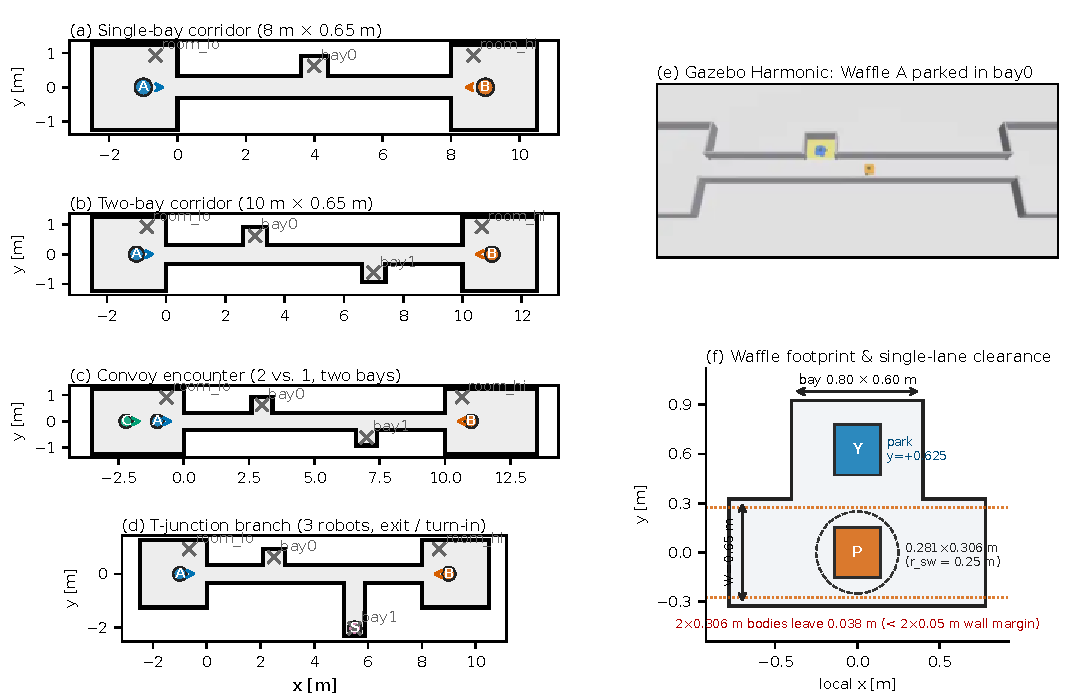
\includegraphics[width=0.71\textwidth]{fig/scenarios.pdf}
\caption{Benchmark topologies and physical envelope. (a)--(d) Top-down 2D layouts (light gray: navigable space; $\times$: discrete refuge parking poses; colored circles/arrows: initial robot poses and travel directions). In (d), the turn-in variant is shown where robot S starts parked in the branch stem (\texttt{bay1}) and robot A's destination is \texttt{bay1}; in the exit variant, A and B traverse end-to-end while S exits \texttt{bay1}. (e) Overhead capture from ROS~2 Jazzy / Gazebo Harmonic showing TurtleBot3 Waffle A parked in \texttt{bay0} while B passes. (f) Cross-sectional clearance geometry showing why two $0.306$\,m-wide Waffles cannot pass side-by-side inside the $0.65$\,m lane.}
\label{fig:scen}
\end{figure*}

All robots follow the physical dimensions and velocity bounds of the ROBOTIS TurtleBot3 Waffle~\cite{turtlebot3} (Fig.~\ref{fig:scen}f): rectangular chassis footprint $0.281\times 0.306$\,m ($[-0.2045,+0.0765]\times[-0.153,+0.153]$\,m relative to the wheel-axle \texttt{base\_footprint}), in-place rotational swept radius $R_{\mathrm{sw}}=0.25$\,m, maximum forward speed $v_{\max}=0.26$\,m/s, asymmetric maximum reverse speed $v_{\mathrm{rev}}=0.15$\,m/s, angular velocity bound $\omega_{\max}=1.82$\,rad/s, linear acceleration $a_{\max}=0.5$\,m/s$^2$, angular acceleration $\alpha_{\max}=3.0$\,rad/s$^2$, and $360^\circ$ planar lidar range $R_{\mathrm{lidar}}=3.5$\,m. Two Waffles placed side-by-side occupy $2\times 0.306=0.612$\,m of the $0.65$\,m corridor, leaving $0.038$\,m total---less than the $c_{\mathrm{clear}}=0.05$\,m wall margin required per robot---and the low-level motion controller tracks the corridor centerline $y=0$ without lateral passing maneuvers. Consequently, head-on passage is physically impossible unless one robot parks off-lane.

In the base two-robot encounter, Robot~A starts at $x=-1.0$\,m ($t=0$) heading toward $x_{\mathrm{goal},A}=L+1.0$\,m ($s_A=+1$), while Robot~B starts at $x=L+1.0$\,m heading toward $x_{\mathrm{goal},B}=-1.0$\,m ($s_B=-1$) after a start delay drawn per seed from $U[0,8]$\,s ($U[0,10]$\,s in two-bay sweeps). Because A requires $\sim 35$\,s to clear the corridor while B enters within $\sim 12$\,s, every random draw produces a genuine head-on conflict inside the aisle while varying the exact meeting point relative to the bays. Beyond symmetric single-bay (\texttt{corridor\_single\_bay}) and two-bay (\texttt{corridor\_two\_bays}) layouts, the suite includes heterogeneous urgency/payload/speed configurations (\texttt{corridor\_urgent\_loaded}), a three-robot 2-vs.-1 convoy (\texttt{corridor\_convoy}, Fig.~\ref{fig:scen}c) where follower~C trails leader~A by $1.2$\,m, and two three-robot T-junction scenarios (\texttt{corridor\_tjunction} exit and \texttt{corridor\_tjunction\_goal} turn-in, Fig.~\ref{fig:scen}d) in which a side branch at $x=5.5$\,m is modeled as a $2.0$\,m-deep bay (\texttt{bay1}) rather than an unbounded orthogonal road.

\subsection{Broadcast Communication Model}
Robots communicate over a shared local broadcast bus without central routing. Each transmitted packet is scheduled for delivery to every other robot independently with one-way latency $\tau + \delta$, where $\tau\ge 0$ is a fixed base delay (default $\tau=0.05$\,s) and $\delta\sim U[0,j]$ is uniform packet jitter (default $j=0.02$\,s), and is dropped independently per receiver with probability $p_{\mathrm{loss}}\in[0,0.99]$ (default $0\%$). Non-communicating runs (\texttt{reactive}) disable both transmission and reception entirely.

\subsection{Simulator-Agnostic Agent State Machine and Safeguards}\label{sec:proto}
A core architectural principle of the benchmark is zero code divergence between fast Monte Carlo sweeps and 3D ROS~2 execution: each robot instantiates the exact same Python \texttt{Agent} class stepped at $20$\,Hz ($\Delta t=0.05$\,s), receiving pose, filtered lidar points/peer clusters, and bus messages, and returning $(v,\omega)$ unicycle commands plus outgoing JSON dicts. Figure~\ref{fig:proto}a depicts the five-mode state machine (\texttt{CRUISE}, \texttt{NEGOTIATE}, \texttt{YIELD}, \texttt{PROCEED}, \texttt{DONE}) and its fallback transitions.

\begin{figure*}[t]\centering
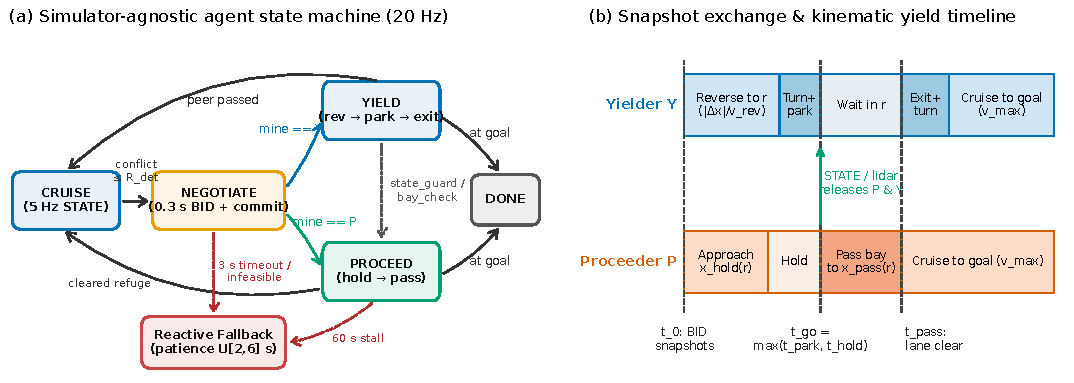
\includegraphics[width=0.74\textwidth]{fig/protocol.pdf}
\caption{Decentralized negotiation architecture. (a) Simulator-agnostic 20\,Hz agent state machine shared identically by \texttt{sim2d} and ROS~2/Gazebo nodes, showing nominal transitions (solid), timeout/infeasibility reactive fallbacks (dashed red), and lossy-channel yield-abort guards (dotted gray). (b) Snapshot exchange and constant-speed kinematic timeline (Eq.~\ref{eq:timeline}) used by \cb, \gb, and Clarke-pivot policies to predict yielder ($Y$) and proceeder ($P$) delays.}
\label{fig:proto}
\end{figure*}

\smallskip\noindent\emph{Conflict Detection and Deterministic Snapshot Resolution:} While driving, negotiating robots broadcast compact \texttt{STATE} beacons at $5$\,Hz containing pose, velocity, active mode, target refuge, and corridor entry timestamp $t_{\mathrm{enter}}$. Peer \texttt{STATE} records remain \emph{fresh} for $\tau_{\mathrm{state}}=1.0$\,s from receipt. Unlike the reactive baseline, negotiating robots detect oncoming conflicts via radio \texttt{STATE} positions whenever an opposing peer lies ahead within longitudinal range $R_{\mathrm{det}}$ (default $6.0$\,m, intentionally exceeding the $3.5$\,m lidar range so negotiation precedes physical proximity). Upon conflict detection, each robot freezes a kinematic \texttt{Snapshot} (pose, speed, direction, goal, $t_{\mathrm{enter}}$, urgency $u_i$, payload flag, kinematic limits, and optional known/blocked refuge IDs or convoy follower snapshots) and broadcasts it inside a \texttt{BID} message, retransmitting every $0.3$\,s. Because every negotiating policy is a pure deterministic function of the sorted snapshot pair and shared map, once both robots hold identical snapshot pairs they compute the exact same \texttt{(yielder, proceeder, refuge)} plan locally without requiring a third arbitration message.

\smallskip\noindent\emph{Lossy-Channel Safeguards and Liveness Timers:} Under packet drops or high latency, two robots may evaluate decisions on asymmetric snapshots (e.g., different map knowledge or one robot timing out first). Three modular safeguards---each individually switchable in \texttt{AgentParams} for factorial ablation---mitigate inconsistent execution:
\begin{itemize}
\item \emph{Commit handshake (\texttt{commit}):} Each robot includes its computed decision in outgoing \texttt{BID}s and delays acting until a peer \texttt{BID} confirms receipt; if decisions conflict, both adopt the lower-ID robot's decision, and unconfirmed commits expire after $3.0$\,s.
\item \emph{State guard (\texttt{state\_guard}):} A yielding robot continuously monitors fresh peer \texttt{STATE} beacons; if its peer is simultaneously yielding into the same bay or yielding to it, the robot aborts its yield and transitions to \texttt{PROCEED}.
\item \emph{Lidar bay check (\texttt{bay\_check}):} Any bay containing a lidar return within $0.45$\,m of its parking pose is marked occupied during planning, and a yielder discovering a robot inside its target bay aborts and proceeds.
\end{itemize}
Complementing these guards, a \texttt{PROCEED} robot triggers renegotiation if fresh \texttt{STATE} shows its designated yielder still cruising toward it, and passes once fresh \texttt{STATE} or lidar confirms the yielder has cleared the lane. A parked yielder exits its bay once peer \texttt{STATE} confirms passage; if \texttt{STATE} is stale under heavy loss, it exits once lidar shows the peer past, or after a randomized park hold $U[6,12]$\,s provided lidar shows the lane clear. Finally, if no peer \texttt{BID} arrives within $\tau_{\mathrm{neg}}=3.0$\,s, or a \texttt{PROCEED} robot stalls for $\tau_{\mathrm{proc}}=60.0$\,s, the agent drops into reactive backoff (re-entering negotiation if a peer \texttt{BID} later arrives); if no feasible refuge exists, it backs off reactively and suppresses renegotiation with that peer for $10.0$\,s. We emphasize that this protocol carries no formal safety or liveness proof; its empirical envelope and transient mutual-yield behavior are audited in Sec.~\ref{sec:rq3}.

\smallskip\noindent\emph{Map-Uncertainty and Multi-Robot Protocol Extensions:} Five targeted protocol extensions support imperfect maps and three-robot encounters: (i)~\texttt{share\_map} piggybacks the sender's known bay IDs on every \texttt{BID} so receivers union them into their local map prior to calling \texttt{decide()}; (ii)~\texttt{explore} initializes robots knowing only end rooms, discovering bays geometrically when within $3.5$\,m lidar range, optionally gating map transmission on physical lidar peer detection (\texttt{share\_on\_detect}) and postponing the decision up to $15.0$\,s until peer detection plus map receipt (\texttt{hold\_for\_map}); (iii)~\texttt{refuge\_blocked} cross-checks lidar bay occupancy against fresh peer \texttt{STATE} poses so static physical obstructions (pallets/closed bays) are broadcast as permanently blocked rather than mistaken for parked peers; (iv)~convoy \texttt{make\_room} commands a same-direction follower blocking a reversing yielder to yield into its own behind-refuge; and (v)~T-junction \texttt{goal\_wait} directs a branch-bound robot whose target stem is occupied to wait off-lane in an upstream bay rather than blocking the main corridor.

\subsection{Dual Simulator Hosts: Fast 2D vs.\ ROS~2 / Gazebo Harmonic}
The benchmark provides two interchangeable execution hosts:
\begin{enumerate}
\item \emph{Fast 2D Unicycle Simulator (\texttt{sim2d}):} Integrates $(x,y,\theta,v,\omega)$ via forward Euler at $20$\,Hz under exact velocity and acceleration saturation, models lidar peer perception as unoccluded $0.25$\,m circles within $3.5$\,m, and checks collisions at every step via exact Separating Axis Theorem (SAT) overlap of the $0.281\times 0.306$\,m Waffle footprints (plus a $0.50$\,m center-distance check against static bay obstacles). Running $>500\times$ faster than real time, \texttt{sim2d} enables multi-thousand-episode factorial sweeps.
\item \emph{ROS~2 Jazzy \& Gazebo Harmonic (\texttt{ros2\_ws}):} Automatically compiles any YAML scenario into an SDF world with 3D wall geometry, optional static box obstacles, and standard TurtleBot3 Waffle models equipped with differential-drive physics and $360^\circ$ GPU planar lidar~\cite{gazebosim}. Each robot runs in an isolated \texttt{agent\_node} that reads ground-truth Gazebo pose (isolating negotiation and lidar-perception transfer from SLAM drift) and raw \texttt{LaserScan} rays, filters out static corridor walls ($>0.12$\,m threshold), clusters remaining returns ($0.35$\,m linkage) into perceived obstacles and peer positions, and exchanges JSON packets over \texttt{/amr\_negotiation/bus} through emulated latency, jitter, and per-receiver loss. An independent \texttt{referee\_node} logs identical episode metrics and SAT body-overlap checks.
\end{enumerate}

\section{Negotiation Policies, Kinematic Cost Model, and Mechanism Design}\label{sec:pol}

Table~\ref{tab:taxonomy} summarizes the nine policy variants compared across our studies. All negotiating policies operate on the frozen snapshot pair $(S_A, S_B)$ and select a yielder $Y\in\{A,B\}$ and a feasible refuge $r\in\mathcal{F}(Y,P)$.

\begin{table*}[t]\centering
\caption{Taxonomy of benchmarked corridor coordination policies across communication, information inputs, model assumptions, and strategic properties.}
\label{tab:taxonomy}
{\footnotesize\setlength{\tabcolsep}{2.9pt}
\begin{tabular}{@{}llcccc>{\raggedright\arraybackslash}p{0.190\textwidth}@{}}\toprule
Policy (Code) & Family & Comms & State Inputs Used & Motion Model & Incentive Prop. & Multi-Robot / Map Scope \\\midrule
\texttt{reactive} (R) & Local sensor backoff & None & $3.5$\,m lidar proximity & None & N/A & Pairwise/local; patience $U[2,6]$\,s \\
\texttt{reservation} (S) & Corridor mutex lock & \texttt{STATE} & Occupancy, $t_{\mathrm{enter}}$ & None & First-in wins & Corridor FCFS; rulebook inside-tie \\
\texttt{fixed\_priority} (F) & Static social law & \texttt{STATE}+\texttt{BID} & Robot ID, feasibility & Feasibility only & Non-manipulable$^\dagger$ & Pairwise + \texttt{make\_room} / \texttt{goal\_wait} \\
\texttt{rules\_default} (D) & Lexicographic rules & \texttt{STATE}+\texttt{BID} & $u_i$, load, $t_{\mathrm{enter}}$, bay $\le 2$\,m & Feasibility only & Non-manipulable$^\dagger$ & Ordered 6-rule industrial etiquette \\
\texttt{rules\_proximity} (P) & Geometric rulebook & \texttt{STATE}+\texttt{BID} & Nearest-bay $|x_r - x_i|$, D & Refuge distance & Pose-dependent & Closest-refuge ahead of seniority \\
\texttt{learned} (L) & Tabular bandit & \texttt{STATE}+\texttt{BID} & Binned bay dist., $u_i$, load & Offline sim table & Co-op assumed & 93 states; unseen $\to$ fixed priority \\
\cb\ (C) & Kinematic auction & \texttt{STATE}+\texttt{BID} & Full \texttt{Snapshot}, $u_i$ & Constant-speed & Manipulable & Pairwise social-cost minimization \\
\gb\ (G) & Convoy auction & \texttt{STATE}+\texttt{BID} & Group \texttt{Snapshot}s & Side-level sum & Co-op assumed & Distinct bays across convoy group \\
\texttt{clarke} (V) & VCG mechanism & \texttt{STATE}+\texttt{BID} & Cost vectors $r_i(o)$ & Constant-speed & DSIC (unilat.)$^\ddagger$ & Externality payment to fleet bank \\\bottomrule
\end{tabular}}\\[2pt]
{\footnotesize $^\dagger$Non-manipulable with respect to cost bids; physical state claims ($u_i$, load, known bays) are assumed authentic. $^\ddagger$Dominant-strategy incentive compatible for unilateral cost scaling under the shared kinematic model; runs a budget surplus and does not prevent joint shading or bay-set omission.}
\end{table*}

\subsection{Non-Communicating, Lock, and Heuristic Rulebook Policies}
\smallskip\noindent\emph{Reactive Baseline (\texttt{reactive}, R):} Transmits and processes no radio messages. When lidar detects an obstacle ahead within stopping distance in the lane, the robot halts, waits out a random patience timer drawn per conflict from $U[2,6]$\,s to break symmetry, and if still blocked reverses into the nearest refuge behind its current $x$-coordinate.

\smallskip\noindent\emph{Corridor Reservation (\texttt{reservation}, S):} Emulates industrial AGV zone-control locks~\cite{fanti2002event} on a first-come, first-served (FCFS) basis using peer \texttt{STATE} beacons. If an oncoming robot is already inside $[0,L]$ while robot $i$ is still outside, robot $i$ yields preemptively in its end room until the corridor clears. If both robots enter before learning of one another (e.g., near-simultaneous entry or packet delay), they fall back to \texttt{rules\_default}.

\smallskip\noindent\emph{Fixed Priority (\texttt{fixed\_priority}, F) and Rulebooks (D, P):} \texttt{fixed\_priority} always assigns the higher-ID robot ($B$ in $\{A,B\}$) to yield into its lowest-delay feasible refuge, falling back to $A$ only if $B$ has no feasible plan. \texttt{rules\_default} (D) evaluates an ordered six-tier rulebook inspired by industrial AGV conventions and single-track road etiquette~\cite{kato1992coordinating,highwaycode}: (1)~only one robot has a feasible refuge; (2)~urgency difference $|u_A-u_B|\ge 0.5$ (lower urgency yields); (3)~asymmetric payload (unloaded yields to loaded); (4)~corridor seniority $|t_{\mathrm{enter},A}-t_{\mathrm{enter},B}|\ge 1.0$\,s (later entrant yields); (5)~only one robot has a feasible refuge within $2.0$\,m behind it; and (6)~lower-ID priority tie-break. \texttt{rules\_proximity} (P) promotes ``closest feasible refuge yields'' ($||x_{r_A}-x_A|-|x_{r_B}-x_B||\ge 0.1$\,m) immediately after payload and ahead of corridor seniority.

\subsection{Kinematic Yield-Plan Model, \cb, and Convoy \gb}
To price candidate yield plans quickly and deterministically on embedded CPUs, \texttt{planner.py} evaluates a constant-speed kinematic timeline (Fig.~\ref{fig:proto}b) that uses exact robot speed bounds and refuge coordinates while intentionally omitting acceleration ramps and steering transients. For candidate yielder $Y$, proceeder $P$ (with travel directions $s_Y,s_P\in\{-1,+1\}$), and refuge $r\in\mathcal{R}$, the proceeder's braking stop coordinate, lane hold point, and clearance point are
\begin{equation}
\begin{aligned}
x_{\mathrm{stop}}(P) &= x_P + s_P \frac{\max(0, v_P)^2}{2 a_{\max,P}}, \\
x_{\mathrm{hold}}(r, P) &= x_r - s_P \Bigl(\frac{w_r}{2} + R_{\mathrm{sw}} + c_{\mathrm{clear}}\Bigr), \\
x_{\mathrm{pass}}(r, P) &= x_r + s_P \Bigl(\frac{w_r}{2} + R_{\mathrm{sw}} + c_{\mathrm{clear}}\Bigr).
\end{aligned}
\label{eq:geom}
\end{equation}
Refuge $r$ belongs to the feasible set $\mathcal{F}(Y,P)$ iff $P$ can stop before $x_{\mathrm{hold}}$, $P$'s goal lies at or beyond $x_{\mathrm{pass}}$, and $Y$'s goal lies at or beyond $x_r$: $s_P(x_{\mathrm{hold}}-x_{\mathrm{stop}}(P))\ge 0$, $s_P(x_{\mathrm{goal},P}-x_{\mathrm{pass}})\ge 0$, and $s_Y(x_{\mathrm{goal},Y}-x_r)\ge 0$.

Let $t_{\mathrm{turn}} = \frac{\pi/2}{0.8\,\omega_{\max,Y}}$ denote an effective $90^\circ$ turn duration and $v_Y^{\mathrm{app}} = v_{\mathrm{rev},Y}$ if $s_Y(x_r-x_Y)<0$ (reversing to a behind-refuge) and $v_{\max,Y}$ otherwise. The predicted synchronization times and free-flow-subtracted delays $d_Y(r), d_P(r)$ are
\begin{equation}
\begin{aligned}
t_{\mathrm{park}} &= \frac{|x_r - x_Y|}{v_Y^{\mathrm{app}}} + t_{\mathrm{turn}} + \frac{|y_{\mathrm{park},r}|}{v_{\max,Y}}, \\
t_{\mathrm{pass}} &= \max\!\Bigl(t_{\mathrm{park}},\, \frac{|x_{\mathrm{hold}} - x_P|}{v_{\max,P}}\Bigr) + \frac{|x_{\mathrm{pass}} - x_{\mathrm{hold}}|}{v_{\max,P}}, \\
d_Y(r) &= t_{\mathrm{pass}} + \frac{|y_{\mathrm{park},r}|}{v_{\mathrm{rev},Y}} + t_{\mathrm{turn}} \\
&\quad + \frac{|x_{\mathrm{goal},Y} - x_r| - |x_{\mathrm{goal},Y} - x_Y|}{v_{\max,Y}}, \\
d_P(r) &= t_{\mathrm{pass}} + \frac{|x_{\mathrm{goal},P} - x_{\mathrm{pass}}| - |x_{\mathrm{goal},P} - x_P|}{v_{\max,P}}.
\end{aligned}
\label{eq:timeline}
\end{equation}
Each candidate yielder $Y$ selects its best feasible refuge $r^\ast(Y,P)=\arg\min_{r\in\mathcal{F}(Y,P)}[d_Y(r)+d_P(r)]$ (ties broken by $|x_r-x_Y|$). Under \cb\ (C), each side's urgency-weighted social cost is evaluated---optionally perturbed in study \texttt{S7} by a multiplicative log-normal estimation error seeded deterministically on \texttt{(seed, robot\_id, round(t,1))} so both robots observe identical noisy bids---and the lower-cost yielder is selected:
\begin{equation}
\begin{aligned}
\tilde{c}_Y &= \bigl(u_Y d_Y(r^\ast) + u_P d_P(r^\ast)\bigr)\exp(\sigma \epsilon_Y), \\
Y^\ast &= \arg\min_{Y\in\{A,B\}} \tilde{c}_Y,
\end{aligned}
\label{eq:costbid}
\end{equation}
where $\epsilon_Y\sim\mathcal{N}(0,1)$ and $\tilde{c}_Y=\infty$ if $\mathcal{F}(Y,P)=\emptyset$.

For three-robot convoys, pairwise \cb\ negotiates only between opposing leaders $A$ and $B$, ignoring trailing follower $C$. Our side-level extension \gb\ (G) attaches same-direction followers' snapshots to the leader's \texttt{BID} ($\mathcal{G}_Y$ vs.\ $\mathcal{G}_P$), assigns distinct bays greedily across $y\in\mathcal{G}_Y$ (while allowing end rooms to be shared), and evaluates the side cost
\begin{equation}
\begin{aligned}
C_{\mathrm{grp}}(\mathcal{G}_Y,\mathcal{G}_P) &= \sum_{y\in\mathcal{G}_Y} u_y d_y(r_y^\ast) + \Bigl(\max_{f\in\mathcal{G}_P\setminus\{P\}}\frac{|x_f-x_P|}{v_{\max,f}}\Bigr)\!\sum_{y\in\mathcal{G}_Y} u_y \\
&\quad + \Bigl(\max_{y\in\mathcal{G}_Y} d_{P,y}(r_y^\ast)\Bigr)\!\sum_{p\in\mathcal{G}_P} u_p.
\end{aligned}
\label{eq:groupbid}
\end{equation}
Notice that Eq.~\eqref{eq:groupbid} evaluates each yielding member's $d_y(r_y^\ast)$ independently; as Sec.~\ref{sec:rq4} demonstrates, when a trailing follower must first clear the lane via \texttt{make\_room} before the leader can reverse past it, this additive approximation underestimates the serial convoy yield time.

\subsection{Clarke-Pivot (VCG) Mechanism and Repeated Fairness Credit}
Under unpriced \cb~\eqref{eq:costbid}, a self-interested robot can inflate its bid so its opponent always yields. Conversely, under a naive direct transfer where the proceeder pays the yielder's reported bid, a robot can shade its report downward to win a favorable role or extract excess transfer. To restore dominant-strategy truthfulness over the two outcomes $o\in\{A,B\}$ (named by who yields), the Clarke-pivot mechanism (\texttt{clarke}, V)~\cite{clarke1971multipart} elicits each robot's reported weighted-delay vector $r_i(o)$ (truthfully $c_i(o)=u_i d_i(r^\ast(o))$), chooses the social-cost-minimizing outcome $o^\ast$, and charges each robot the externality pivot payment $p_i$ to an external fleet bank:
\begin{equation}
\begin{aligned}
o^\ast &= \arg\min_{o\in\{A,B\}} \sum_{i\in\{A,B\}} r_i(o), \\
p_i &= \sum_{j\neq i} r_j(o^\ast) - \min_{o\in\{A,B\}} \sum_{j\neq i} r_j(o) \ge 0.
\end{aligned}
\label{eq:clarke}
\end{equation}
With two robots, $p_i$ reduces to a second-price rule on the opponent's cost difference: if $i$'s report flips the decision against $j$'s preference, $i$ pays $|r_j(A)-r_j(B)|$; otherwise $p_i=0$. Robot $i$'s quasi-linear single-encounter utility is $U_i = -u_i d_i^{\mathrm{real}}(o^\ast) - p_i$, settled in virtual delay-seconds per encounter without inter-encounter carry-over.

When robots belong to a single cooperative fleet but encounter each other repeatedly across $t=1,\dots,K$ episodes, static tie-breaking (\texttt{fixed\_priority}) imposes chronic delay asymmetry on higher-ID robots. Following karma-inspired non-monetary credit allocation~\cite{censi2019karma,elokda2024karma}, we evaluate a cumulative-delay fairness rule parameterized by weight $\lambda\ge 0$:
\begin{equation}
\begin{aligned}
o_t^\ast &= \arg\min_{o\in\{A,B\}} \Bigl[d_{A,t}(o)+d_{B,t}(o) \\
&\quad + \lambda\bigl|(D_{A,t-1}^{\mathrm{cum}}+d_{A,t}(o)) - (D_{B,t-1}^{\mathrm{cum}}+d_{B,t}(o))\bigr|\Bigr],
\end{aligned}
\label{eq:karma}
\end{equation}
where $D_{i,t}^{\mathrm{cum}} = \sum_{\tau=1}^{t}\max(0, d_{i,\tau}(o_\tau^\ast))$, and cumulative equity is scored via Jain's fairness index~\cite{jain1984fairness}, $J(D_A^{\mathrm{cum}},D_B^{\mathrm{cum}}) = (D_A^{\mathrm{cum}}+D_B^{\mathrm{cum}})^2 / [2((D_A^{\mathrm{cum}})^2+(D_B^{\mathrm{cum}})^2)] \in [0.5, 1]$.

\subsection{Outcome-Trained Tabular Contextual Bandit (\texttt{learned}, L)}
To test whether a planner-free policy can learn refuge selection directly from simulated outcomes without explicit kinematic equations, \texttt{learned} discretizes each conflict into a 5-tuple feature key: each robot's nearest feasible behind-refuge distance binned at $\{1.0, 2.5, 5.0\}$\,m (plus bin~4 for none), urgency ordering $\mathrm{sign}(u_A-u_B)\in\{-1,0,+1\}$, and binary payload flags $(l_A,l_B)$. Trained centrally offline on $800$ two-bay encounters by executing both forced outcomes ($1,600$ episodes; $93$ populated keys), the policy selects the side with lower empirical mean weighted delay and falls back to \texttt{fixed\_priority} on unseen keys. It serves as a transparent tabular contextual bandit baseline rather than deep MARL.

\section{Experimental Design and Statistical Methodology}\label{sec:exp}

\subsection{Metrics and Paired Hindsight Reference}
Every episode runs until all robots reach their goals or the universal time limit $T_{\max}=180.0$\,s expires. We record: (1)~\emph{success} (all goals reached within $180$\,s with zero collisions); (2)~\emph{deadlock} ($t=180$\,s reached without collision); (3)~\emph{collision} (any SAT overlap of Waffle chassis rectangles, or center within $0.50$\,m of a blocked-bay obstacle; note that the released \texttt{min\_clearance} diagnostic column reports axle-to-axle distance minus $2R_{\mathrm{sw}}=0.50$\,m, which can turn slightly negative when two Waffles stop nose-to-nose without chassis contact because the front bumper extends only $0.0765$\,m ahead of the axle); (4)~free-flow-subtracted \emph{delay} $D = \sum_i w_i(T_i - T_i^{\mathrm{free}})$, where $T_i^{\mathrm{free}}$ is robot $i$'s solo corridor traversal time and $w_i=1$ (total delay) or $w_i=u_i$ (urgency-weighted delay); (5)~\emph{reverse distance} traveled; and (6)~\emph{first-yielder identity}.

Raw delay $D$ conflates policy suboptimality with irreducible encounter geometry (e.g., two robots meeting far from any bay must incur delay under \emph{any} policy). For every two-robot encounter $k$, we therefore run both forced yield outcomes---\texttt{forced\_A} ($A$ yields into its best feasible refuge) and \texttt{forced\_B} ($B$ yields)---defining the hindsight \emph{best forced yielder} reference $\min(D_A^{(k)}, D_B^{(k)})$ (\texttt{oracle} O for $w_i=1$, \texttt{oracle\_w} O$_w$ for $w_i=u_i$). Policy $\pi$'s paired \emph{excess delay} across $N$ encounters is
\begin{equation}
\Delta_\pi = \frac{1}{N}\sum_{k=1}^{N}\Bigl(D_\pi^{(k)} - \min\bigl(D_A^{(k)}, D_B^{(k)}\bigr)\Bigr).
\label{eq:excess}
\end{equation}
$\Delta_\pi=0$ indicates that $\pi$ matched the better forced yield decision on every encounter. Because the reference optimizes only \emph{who} yields under immediate execution rather than full continuous trajectory timing, a policy that alters conflict timing (such as \texttt{hold\_for\_map}) can occasionally record $\Delta_\pi<0$. We refer to $\Delta_\pi$ as excess delay rather than ``regret'' to avoid ambiguity between online-learning cumulative regret and mechanism-design ex-post regret. For 2-vs.-1 convoys, an analogous \texttt{side\_oracle} takes the minimum of forcing the convoy side vs.\ the lone robot to yield.

\subsection{Factorial Study Suite, Provenance, and Statistical Reporting}
Table~\ref{tab:design} details all 18 2D factorial studies (50,374 simulated episodes, counting each hindsight reference evaluation once though it executes two forced runs) plus the 496 seed-paired ROS~2 / Gazebo runs (460 main validation runs across every study plus 36 hold/share-on-detect runs), grouped by RQ1--RQ4. Per-episode CSV tables and reproduction scripts for all studies---including the 1,080 convoy and 384 T-junction episodes---are released in the benchmark archive.

\begin{table*}[t]\centering
\caption{Complete experimental design grouped by research question. Unless stated otherwise, B's start delay is drawn per seed from $U[0,8]$\,s, base latency is $\tau=0.05$\,s with $0.02$\,s jitter, packet loss is $0\%$, conflict range is $R_{\mathrm{det}}=6.0$\,m, and $v_{\max}=0.26$\,m/s.}
\label{tab:design}
{\footnotesize\setlength{\tabcolsep}{3.4pt}
\begin{tabular}{@{}ll>{\raggedright\arraybackslash}p{0.35\textwidth}rlr@{}}\toprule
Layer / RQ & Study (Sec.) & Factorial Grid Factors & Seeds & Policies Evaluated & $N$ \\\midrule
\multirow{6}{*}{RQ1 (Sec.~\ref{sec:rq1})}
 & Single bay (\texttt{S1}) & Bay $x\in\{1,2,3,4,5,6,7\}$\,m & 60 & R, F, D, P, C, O, O$_w$ & 2,940 \\
 & Zone reservation & Bay $x\in\{1,\dots,7\}$\,m (separate 30-seed draw set) & 30 & S, F, D, C, forced A/B & 1,260 \\
 & Two bays (\texttt{S4}) & Bay 1 $\{2,3,4\}\times$ Bay 2 $\{6,7,8\}$\,m $\times$ side; B $U[0,10]$\,s & 20 & R, F, D, P, C, O, O$_w$ & 2,520 \\
 & Asymmetric robots (\texttt{S2}) & $u_B\in\{1,3\}\times$ load $\{0,1\}\times v_B\in\{0.26,0.13\}$\,m/s $\times$ bay $\{2,4,6\}$\,m & 30 & R, F, D, P, C, O, O$_w$ & 5,040 \\
 & Noisy bids (\texttt{S7}) & $\sigma\in\{0,0.1,0.25,0.5,1.0\}\times$ bay $x\in\{1,\dots,7\}$\,m & 30 & C, P, O & 3,150 \\
 & Learned bandit & Train: 800 two-bay pairs; Eval: 150 ID + 150 OOD & -- & L, F, D, C, O$_w$ & 1,600+1,500 \\\midrule
\multirow{3}{*}{RQ2 (Sec.~\ref{sec:rq2})}
 & Unpriced misreport (\texttt{S6}) & B bid scale $k\in\{1,1.5,2,4,10\}\times$ bay $x\in\{2,4,6\}$\,m & 60 & C, O & 1,080 \\
 & Clarke VCG (\texttt{S9}) & Deviator $\{\text{A, B, AB}\}\times 10$ scales $k\in[0.25,4]\times u_B\{1,3\}\times$ bay $\{2,4,6\}$ & 60 & V (+ none/naive eval) & 10,080 \\
 & Repeated fairness (\texttt{S10}) & 50 sequences $\times$ 20 encounters, bay $U[1,7]$\,m; $\lambda\in\{0,0.25,0.5,1,2\}$ & -- & forced A/B (offline) & 2,000 \\\midrule
\multirow{7}{*}{RQ3 (Sec.~\ref{sec:rq3})}
 & Comms sweep (\texttt{S3}) & Loss $\{0,10,30,50,70,90\}\%\times\tau\in\{0.05,0.25,0.5,1,2\}$\,s & 30 & F, D, P, C & 3,600 \\
 & Comms stress (\texttt{S8}) & $R_{\mathrm{det}}\{6,3,1.5\}$\,m $\times v\{0.26,0.5\}$\,m/s $\times$ loss $\{0,50,90\}\%\times\tau\{0.05,0.5,2\}$\,s & 20 & F, D, P, C & 4,320 \\
 & Extreme comms (\texttt{S8b}) & $R_{\mathrm{det}}\in\{1.5,6\}$\,m $\times$ loss $\{90,97,99\}\%\times\tau\in\{2,4,8\}$\,s; $v=0.5$\,m/s & 20 & F, D, P, C & 1,440 \\
 & Safeguard ablation (\texttt{S8c}) & \texttt{S8b} grid $\times$ \texttt{commit} $\{0,1\}\times$ \texttt{state\_guard} $\{0,1\}\times$ \texttt{bay\_check} $\{0,1\}$ & 20 & F, C & 5,760 \\
 & Asymmetric maps & 7 bay-knowledge splits $\times$ \texttt{share\_map} $\{0,1\}\times$ loss $\{0,50\}\%$; bays $3,7$\,m & 10 & F, D, C & 840 \\
 & Blocked bays & Physically obstructed bays $\in\{\emptyset,\text{bay0},\text{bay1},\text{both}\}\times$ loss $\{0,50\}\%$ & 10 & R, F, D, C & 320 \\
 & Explore \& hold & 4 map modes $\times R_{\mathrm{det}}\in\{6,3.5\}$\,m $\times$ loss $\{0,50\}\%$ (+ hold batch) & 30 & F, D, C & 1,440+360 \\\midrule
\multirow{3}{*}{RQ4 (Sec.~\ref{sec:rq4})}
 & Convoy 2 vs.\ 1 & B type (equal, loaded, $u_B=3$) $\times$ bays $\{2,4\}\times\{6,8\}\times$ delay $\{0,4,8\}\times$ loss & 3 & F, D, C, G, side ref. & 1,080 \\
 & T-junction (3 robots) & Delays $(A,B,S)\in\{0,4\}\times\{0,4,8\}\times\{0,6\}$\,s $\times 2$ S goals $\times$ loss $\{0,50\}\%$ & 2 & R, F, D, C & 384 \\
 & ROS~2 / Gazebo 3D & Seed-paired reduced grid across all studies + 36 hold/rerun runs & 6--10 & R, S, F, D, P, L, C, G, V, O & 460+36 \\\bottomrule
\end{tabular}}
\end{table*}

Apart from explicitly noted pre-fix failure counts that motivated protocol additions (6/1,440 pre-fix extreme-loss collisions, pre-\texttt{make\_room} convoy blocks, 19/48 pre-\texttt{goal\_wait} T-junction deadlocks, and 10/10 pre-\texttt{refuge\_blocked} obstacle stalls), all reported statistics reflect the final unified agent codebase; the final two commits adding opt-in explore/hold modes and Gazebo obstacle spawning leave default execution paths unchanged. Each episode seed fixes start delays and channel realizations so policies are evaluated on identical encounters. Delay means are computed over successful episodes only (making delay a conservative lower bound whenever a policy deadlocks). Uncertainties ($\pm$) denote 95\% confidence intervals of the mean (paired per-encounter intervals for $\Delta_\pi$), proportions carry Wilson 95\% intervals, and zero-collision counts report Clopper--Pearson/rule-of-three 95\% upper bounds.

\section{Results I: Information, Geometry, Cost Noise, and Generalization (RQ1)}\label{sec:rq1}

\subsection{The Price of Zero Communication}
In the single-bay baseline (\texttt{S1}: 7 bay positions $\times$ 60 draws = 420 episodes per policy), the non-communicating \texttt{reactive} policy succeeded in $93.8\%$ [91.1--95.7\%] of encounters, deadlocking in the remaining 26 episodes when random patience timers failed to break head-on symmetry before $180$\,s. Even across its 394 successful episodes, \texttt{reactive} averaged $97.0\pm 5.0$\,s total delay versus $26.8\pm 0.6$\,s for the best forced yielder---a $3.6\times$ penalty (or up to $113$\,s, $4.2\times$, if deadlocks are charged at $180$\,s). Without shared intent, both robots initiated simultaneous reverse maneuvers in $39\%$ of episodes, driving $5.7$\,m in reverse per encounter compared with $0.64$\,m under the reference. By contrast, all four negotiating policies in \texttt{S1} (\texttt{fixed\_priority}, \texttt{rules\_default}, \texttt{rules\_proximity}, and \cb) achieved $100\%$ completion (420/420) and zero collisions. Note that \texttt{fixed\_priority} is a static social law that could execute without radio if robot IDs were visually observable; because we did not evaluate message-free ID sensing, the gap over \texttt{reactive} reflects a shared tie-breaking rule together with the broadcast protocol implementing it.

\begin{figure*}[t]\centering
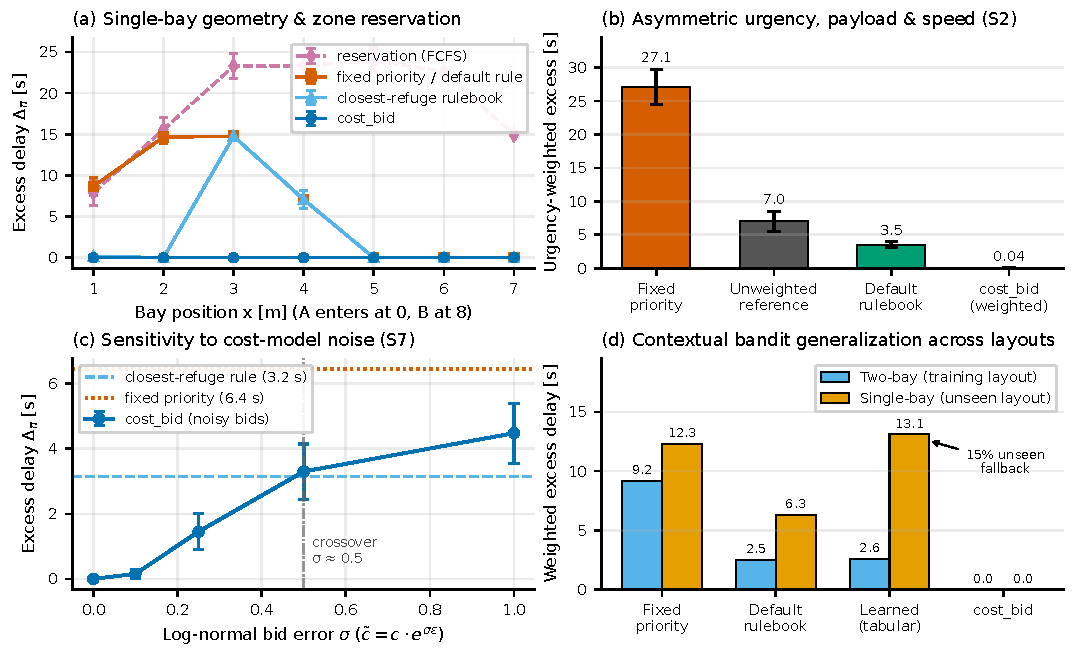
\includegraphics[width=0.71\textwidth]{fig/rq1_information.pdf}
\caption{RQ1---Information fidelity, corridor geometry, estimation noise, and layout generalization. (a) Mean excess delay $\Delta_\pi$~\eqref{eq:excess} vs.\ bay coordinate $x$ in the single-bay corridor (\texttt{S1} and \texttt{reservation}). (b) Urgency-weighted excess delay across heterogeneous urgency, payload, and speed (\texttt{S2}, $N=5{,}040$). (c) Sensitivity of \cb\ to multiplicative log-normal bid noise $\sigma$ (\texttt{S7}, $N=3{,}150$), showing parity with noise-free \texttt{rules\_proximity} at $\sigma\approx 0.5$. (d) Tabular contextual bandit (\texttt{learned}) weighted excess delay on its training two-bay layout vs.\ an unseen single-bay layout. Error bars show 95\% CIs.}
\label{fig:rq1}
\end{figure*}

\subsection{Bay Geometry and Corridor Zone Reservation}
Figure~\ref{fig:rq1}a shows how excess delay $\Delta_\pi$ varies with pull-in bay position $x\in\{1,\dots,7\}$\,m for symmetric robots. Under \texttt{fixed\_priority} and \texttt{rules\_default} (which coincide when robots have equal urgency and load, because $A$ always enters at $t=0$ ahead of delayed $B$), excess delay averages $6.4\pm 0.6$\,s overall, spiking to $14.6$--$14.8$\,s when the bay sits near $A$'s entrance ($x=2$--$3$\,m): $B$ is forced to reverse all the way back to \texttt{room\_hi} even when $A$ has just passed a nearby bay. Promoting geometric proximity ahead of corridor seniority (\texttt{rules\_proximity}) halves overall excess delay to $3.1\pm 0.5$\,s, leaving a residual peak only at $x=3$\,m where $A$ has slightly passed the bay at conflict detection yet reversing $A$ into it remains cheaper than reversing $B$ out of the aisle.

First-come corridor mutex locking (\texttt{reservation}, evaluated over 210 encounters across $x\in\{1,\dots,7\}$\,m) completed 100\% of episodes without collision, but incurred $18.8\pm 0.9$\,s excess delay---nearly triple \texttt{fixed\_priority} ($6.5\pm 0.9$\,s on the same draws)---and beat the best forced yielder in $0/210$ encounters. Because $B$'s start pose lies on $A$'s exit centerline, holding outside the aisle requires $B$ to turn and park off-lane inside \texttt{room\_hi} ($\sim 17$\,s maneuver overhead) while waiting out $A$'s entire corridor traversal rather than exploiting intermediate bays. Layouts whose staging queues already sit off the exit lane would penalize reservation less severely.

Across all 420 single-bay (\texttt{S1}) and 360 two-bay (\texttt{S4}) encounters per policy, noise-free \cb\ selected the exact same yielder as the hindsight reference in $100\%$ of episodes ($\Delta_\pi = 0.0$\,s). Because \cb\ uses the simulator's true speed limits and refuge coordinates while the simulator is deterministic, this exact agreement primarily validates the planning pipeline: omitting acceleration and turn transients causes a $1.9$\,s per-robot mean absolute prediction error (maximum $4.0$\,s across 780 episodes), yet in symmetric corridors that error never flips the discrete ordinal comparison between $A$ and $B$.

\subsection{Heterogeneous Fleet Asymmetry and Objective Alignment}
When robots differ in task urgency ($u_B\in\{1,3\}$), payload status, and speed limit ($v_B\in\{0.26,0.13\}$\,m/s; \texttt{S2}, 5,040 episodes, Fig.~\ref{fig:rq1}b), static ID priority breaks down severely, incurring $27.1\pm 2.6$\,s urgency-weighted excess delay because high-urgency or slow $B$ is forced into long reverse maneuvers. Incorporating urgency and load rules (\texttt{rules\_default}) cuts weighted excess nearly eightfold to $3.5\pm 0.4$\,s. Crucially, the hindsight reference that minimizes \emph{unweighted} total delay (\texttt{oracle}) still suffers $7.0\pm 1.5$\,s urgency-weighted excess---demonstrating that optimizing the wrong fleet objective costs twice as much as replacing kinematic planning with a heuristic rulebook. Urgency-weighted \cb\ achieves $\Delta_\pi = 0.04\pm 0.02$\,s, matching \texttt{oracle\_w} in $98\%$ of encounters (704/720). Inspecting the 16 disagreed episodes confirms that all are genuine near-ties where omitted acceleration transients tip the balance: their predicted bid gap has a median of just $0.6$\,s (maximum $2.2$\,s), compared with $12.4$\,s across the 704 agreed encounters.

\subsection{Cost-Model Noise Crossover and Bandit Layout Shift}
Real fleets face travel-time uncertainty from floor friction, battery sag, and localization jitter. Perturbing each bid by log-normal multiplicative noise $e^{\sigma\epsilon}$ (\texttt{S7}, Fig.~\ref{fig:rq1}c) raises \cb\ excess delay from $0.0$\,s ($\sigma=0$) to $0.2\pm 0.1$\,s ($\sigma=0.1$), $1.5\pm 0.6$\,s ($\sigma=0.25$), $3.3\pm 0.8$\,s ($\sigma=0.5$), and $4.5\pm 0.9$\,s ($\sigma=1.0$). At $\sigma=0.5$ (a typical multiplicative factor of $e^{0.5}\approx 1.65\times$), noisy \cb\ offers no statistical advantage over noise-free \texttt{rules\_proximity} ($3.2\pm 0.8$\,s on the same draws), remaining clearly superior only for $\sigma\le 0.25$. Note that \texttt{S7} perturbs scalar bid totals; systematic structural biases (e.g., miscalibrated $v_{\mathrm{rev}}$) remain an open test.

Similarly, the outcome-trained tabular bandit (\texttt{learned}, Fig.~\ref{fig:rq1}d) matches \texttt{rules\_default} in-distribution on held-out two-bay corridors ($+2.6$\,s vs.\ $+2.5$\,s weighted excess; $\ge 200$ training encounters suffice to plateau within $3.2$\,s), without using an explicit motion model. When evaluated zero-shot on single-bay corridors with randomized bay positions, however, its excess delay jumps to $+13.1$\,s---trailing even \texttt{fixed\_priority} ($+12.3$\,s) and \texttt{rules\_default} ($+6.3$\,s), with $15\%$ of encounters hitting unseen state keys. Because its coarse ego-centric feature bins omit the proceeder's stopping distance relative to each bay, tabular lookup memorizes layout-specific priors rather than transferable encounter physics.

\section{Results II: Strategic Incentives and Repeated-Encounter Fairness (RQ2)}\label{sec:rq2}

\subsection{Manipulability of Unpriced and Naive-Transfer Bidding}
Standard market-based coordination (\cb) assumes honest cost reporting. In study \texttt{S6} (1,080 episodes), when Robot~$B$ unilaterally inflates its reported bid by $k\ge 2\times$ under unpriced lower-bid-yields, $B$ forces $A$ to yield in 100\% of encounters: $B$'s own mean delay drops from $9.1\pm 1.4$\,s to $8.1\pm 1.2$\,s while fleet total delay rises by $+4.9$\,s ($+20\%$). Symmetrically, in \texttt{S9}'s unpriced baseline (dashed orange curve in Fig.~\ref{fig:rq2}a), Robot~$A$ gains up to $+4.74\pm 0.88$\,s of individual utility by inflating its report to $k=4\times$. Replacing unpriced bidding with a naive side-payment in which the proceeder pays the yielder's reported bid does not fix incentives---it merely inverts the profitable lie (dotted purple curve in Fig.~\ref{fig:rq2}a): $A$ gains $+7.54\pm 1.76$\,s by \emph{under-reporting} $k=0.25\times$ to trigger cheap yields or alter transfer terms, while $B$ gains $+0.68$\,s at $k=0.75\times$.

\begin{figure*}[t]\centering
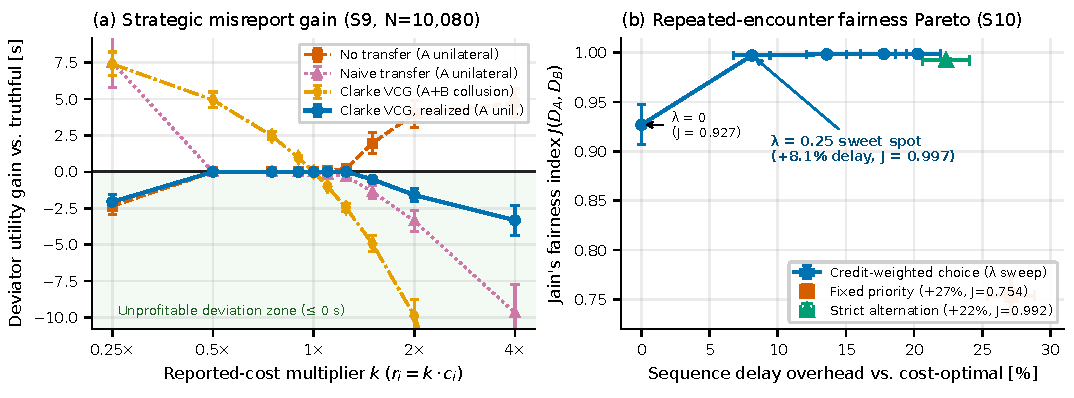
\includegraphics[width=0.74\textwidth]{fig/rq2_incentives.pdf}
\caption{RQ2---Strategic incentives and long-run fairness. (a) Deviator single-encounter utility gain (seconds of urgency-weighted delay plus transfer) relative to truthful reporting ($k=1\times$) across $N=10{,}080$ episodes in \texttt{S9}; values $\le 0$\,s (shaded green) indicate unprofitable deviations. (b) Repeated-encounter Pareto frontier (\texttt{S10}, 50 sequences of 20 encounters) trading sequence delay overhead against cumulative Jain fairness $J(D_A^{\mathrm{cum}}, D_B^{\mathrm{cum}})$ as credit weight $\lambda$~\eqref{eq:karma} varies from $0$ to $2.0$.}
\label{fig:rq2}
\end{figure*}

\subsection{Clarke-Pivot Truthfulness and Its Three Structural Costs}
Study \texttt{S9} evaluates the Clarke-pivot mechanism~\eqref{eq:clarke} across 6 bay/urgency configurations $\times$ 28 unilateral and joint report-scaling profiles ($k\in\{0.25, 0.5, 0.75, 0.9, 1, 1.1, 1.25, 1.5, 2, 4\}$) $\times$ 60 seeds = 10,080 episodes, all succeeding without collision. Under the planner's predicted costs, \emph{zero} unilateral misreport profiles ($0/108$ configuration-scale cells for either $A$ or $B$) improve the deviator's utility ($0.00$\,s max gain), confirming exact dominant-strategy incentive compatibility (DSIC) of the implementation. Evaluated on \emph{realized} simulator trajectories---which differ slightly from predicted timelines due to acceleration and turn transients---unilateral deviations lose up to $-3.3\pm 1.0$\,s at extreme multipliers (solid blue curve in Fig.~\ref{fig:rq2}a), and the largest positive realized gain anywhere on the grid is $+0.02\pm 0.02$\,s (at $k=1.1\times$, statistically indistinguishable from zero).

At the same time, \texttt{S9} exposes three structural limitations that fleet engineers must weigh before deploying VCG:
\begin{enumerate}
\item \emph{Chronic budget surplus:} Consistent with the Green--Laffont theorem~\cite{green1977characterization}, pivot payments must flow to an external sink rather than between the two robots. The bank collects $9.3\pm 1.6$\,s of credit per encounter at $u_B=1$ ($44\%$ of realized social delay) and $10.5\pm 1.5$\,s at $u_B=3$ ($29\%$), requiring periodic lump-sum redistribution outside the encounter loop.
\item \emph{Vulnerability to joint collusion:} If $A$ and $B$ scale their reports down together by the same factor $k<1$, the allocation $o^\ast$ is unchanged while both pivot payments scale by $k$: joint $0.5\times$ shading improves combined utility by $+4.94\pm 0.55$\,s ($+7.42$\,s at $0.25\times$; dash-dotted gold curve in Fig.~\ref{fig:rq2}a).
\item \emph{Participation and non-bid attack surfaces:} Compared against a static \texttt{fixed\_priority} baseline where $A$ never yields and pays zero, $A$ is strictly worse off under Clarke in $100\%$ of encounters (losing $12.1$\,s/encounter at $u_B=1$), so participation requires facility mandate. Moreover, DSIC over cost vectors $r_i(o)$ assumes protocol compliance elsewhere: hiding a known bay from \texttt{BID} shrinks the feasible set $\mathcal{F}$, and spoofing a lower ID exploits \texttt{commit} tie-breaks---manipulations outside VCG's scope.
\end{enumerate}

\subsection{Repeated-Encounter Fairness via Scalar Delay Credit}
In single-owner cooperative fleets, incentives are aligned but repeated static tie-breaking is lopsided: across 50 sequences of 20 random single-bay encounters (\texttt{S10}, Fig.~\ref{fig:rq2}b), \texttt{fixed\_priority} forces $B$ to yield every time, degrading cumulative Jain fairness to $J=0.754$ while inflating total delay by $+27.1\%$ above cost-optimal selection. Notably, pure cost-optimal selection ($\lambda=0$) already achieves $J=0.927$ because random bay positions and entry delays naturally alternate which side is closer to a refuge. Enforcing strict turn-taking (\texttt{alternate}) reaches $J=0.992$ but wastes $+22.3\%$ extra delay by ignoring geometry. Minimizing Eq.~\eqref{eq:karma} at $\lambda=0.25$ hits a sharp Pareto knee: cumulative fairness rises to $J=0.997$ (nearly indistinguishable from equal delay split) at just $+8.1\%$ delay overhead, flipping only near-tie encounters in favor of the robot carrying higher historical delay. We keep this scalar fairness ledger strictly separate from Clarke VCG credit: carrying VCG payments across encounters would turn single-shot externality charges into a dynamic wealth budget, invalidating single-encounter truthfulness.

\section{Results III: Channel Impairment, Safeguard Ablation, and Map Uncertainty (RQ3)}\label{sec:rq3}

\subsection{Packet Loss, Latency, and Factorial Safeguard Ablation}
Across moderate-to-heavy channel degradation---\texttt{S3} (packet loss $0$--$90\%$, latency $0.05$--$2.0$\,s; 3,600 episodes) and \texttt{S8} ($R_{\mathrm{det}}\in\{6,3,1.5\}$\,m, $v_{\max}\in\{0.26,0.5\}$\,m/s, loss up to $90\%$, latency up to $2.0$\,s; 4,320 episodes)---every negotiating policy (\texttt{fixed\_priority}, \texttt{rules\_default}, \texttt{rules\_proximity}, \cb) achieved $\ge 99.3\%$ completion with \emph{zero collisions} (Fig.~\ref{fig:rq3}a). Mean delay remained flat within $1$--$2$\,s up to $50\%$ packet loss because $0.3$\,s \texttt{BID} retransmissions deliver both snapshots well before physical meeting, rising smoothly only above $70\%$ loss as $3.0$\,s negotiation timeouts trigger occasional reactive fallbacks.

\begin{figure*}[t]\centering
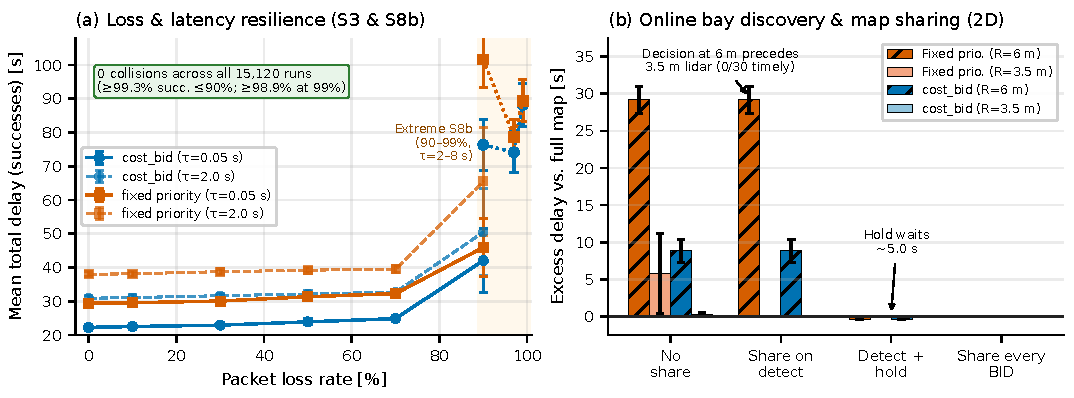
\includegraphics[width=0.74\textwidth]{fig/rq3_comms_maps.pdf}
\caption{RQ3---Resilience to channel impairment and online map uncertainty. (a) Mean total delay over successful episodes across packet loss $0$--$99\%$ and base latency $\tau\in[0.05, 8.0]$\,s (\texttt{S3} at $0.26$\,m/s and extreme \texttt{S8b} shaded right at $0.50$\,m/s); zero collisions occurred across all 15,120 communication-sweep and ablation episodes. (b) Two-bay excess delay relative to full map knowledge in 2D \texttt{explore} mode ($0\%$ loss), showing why \texttt{share\_on\_detect} fails when radio negotiation ($R_{\mathrm{det}}=6$\,m) precedes $3.5$\,m lidar range.}
\label{fig:rq3}
\end{figure*}

Under extreme impairment (\texttt{S8b}: $90$--$99\%$ loss, $2$--$8$\,s latency, $v_{\max}=0.5$\,m/s; 1,440 episodes), an early pre-release version of the agent suffered 6 collisions when both robots yielded on mismatched snapshots and exited simultaneously. After tightening the lane-clearance and park-release transitions in the final protocol, all four policies recorded \emph{zero collisions} across all 1,440 \texttt{S8b} episodes and $98.9$--$99.2\%$ completion. (Note: \texttt{S8b}/\texttt{S8c} ran at $0.5$\,m/s in 2D as a worst-case closing-speed stress test, whereas Gazebo extreme-comms runs used the Waffle's $0.26$\,m/s.)

\begin{table}[t]\centering
\caption{Factorial safeguard ablation (\texttt{S8c}) under 90--99\% packet loss and 2--8\,s latency ($v_{\max}=0.5$\,m/s; 360 episodes per row; \texttt{bay\_check} had zero triggers and identical metrics, so its 8 duplicate rows are condensed). Collisions were 0 in every arm (95\% upper bound 1.06\%).}
\label{tab:abl}
{\footnotesize\setlength{\tabcolsep}{3.4pt}
\begin{tabular}{@{}lccrrrr@{}}\toprule
Policy & \texttt{commit} & \texttt{state} & Succ.\ [\%] & Deadl. & Delay [s] & Dual [\%] \\\midrule
\multirow{4}{*}{\texttt{fixed\_pr.}}
 & \checkmark & \checkmark & 99.2 & 3 & $89.8\pm3.9$ & 21.9 \\
 & \checkmark & --         & 99.2 & 3 & $90.0\pm4.0$ & 23.6 \\
 & --         & \checkmark & 98.1 & 7 & $86.0\pm3.6$ & 15.3 \\
 & --         & --         & 98.6 & 5 & $86.8\pm3.7$ & 16.4 \\\midrule
\multirow{4}{*}{\cb}
 & \checkmark & \checkmark & 98.9 & 4 & $79.6\pm3.9$ & 17.8 \\
 & \checkmark & --         & 99.2 & 3 & $79.9\pm3.9$ & 18.6 \\
 & --         & \checkmark & 99.4 & 2 & $76.4\pm3.7$ & 14.2 \\
 & --         & --         & 99.7 & 1 & $76.8\pm3.7$ & 14.7 \\\bottomrule
\end{tabular}}\\[2pt]
{\footnotesize \texttt{state}: \texttt{state\_guard}. Dual: \% of episodes where both robots entered \texttt{YIELD} before one aborted/exited.}
\end{table}

To isolate which safeguard actually prevents collisions on the final code, study \texttt{S8c} (Table~\ref{tab:abl}, 5,760 episodes) toggles \texttt{commit}, \texttt{state\_guard}, and \texttt{bay\_check} in a full $2^3$ factorial across the \texttt{S8b} grid. Surprisingly, \emph{zero collisions occurred in every single arm}---even with all three safeguards disabled (95\% upper bound $1.06\%$ per 360-episode arm). Two mechanisms explain this negative ablation result. First, at $5$\,Hz beacon rate and $90$--$99\%$ drop probability, a robot lacks any fresh ($<1$\,s) peer \texttt{STATE} with probability $0.90^5=59\%$ to $0.99^5=95\%$, and delivered \texttt{STATE}s are already $2$--$8$\,s old; physical safety is therefore carried by local lidar stopping margins and randomized $U[6,12]$\,s park-release timers rather than radio guards. Second, \texttt{bay\_check} never fired once (all 8 \texttt{bay\_check}-on arms matched \texttt{bay\_check}-off episode-for-episode), while enabling \texttt{commit} added $3.1$--$3.8$\,s of mean delay and actually \emph{increased} transient dual-yield starts ($15.3$--$16.4\% \to 21.9$--$23.6\%$ for \texttt{fixed\_priority}), because holding for a dropped confirmation pushes robots into the $3.0$\,s reactive fallback window. Deadlock differences across arms (1--7 out of 360) lie within sampling noise, and we note that transient mutual yields ($14.2$--$23.6\%$ of runs) carry no analytical termination bound; the tabulated deadlocks represent episodes whose mutual backoff exceeded $180$\,s.

\subsection{Mismatched, Obstructed, and Online-Discovered Bay Maps}
\smallskip\noindent\emph{Static Map Disagreement and Blocked Bays:} When two robots hold different static bay subsets in the two-bay corridor (840 episodes, 10 seeds/cell), no collisions or deadlocks occur because \texttt{commit} resolves mismatched decisions in favor of lower-ID Robot~$A$. Delay rises only when $A$ holds an inferior map: if $A$ knows only \texttt{bay0} ($x=3$\,m), \cb\ loses $+9.1$\,s and \texttt{fixed\_priority}/\texttt{rules\_default} lose $+29.6$\,s ($0\%$ loss) because $B$ is sent all the way to \texttt{room\_hi}; if $A$ knows no bays, all policies lose $+30.9$--$31.1$\,s. Piggybacking known bay IDs in every \texttt{BID} (\texttt{share\_map}) eliminates $100\%$ of this excess delay ($+0.0$\,s) whenever at least one robot knows a bay, even under $50\%$ packet loss. Conversely, when a mapped bay is physically blocked by an unmapped pallet (320 episodes), naive \texttt{bay\_check} deadlocked $10/10$ runs by mistaking the static obstacle for a yielded peer; cross-checking against fresh \texttt{STATE} beacons (\texttt{refuge\_blocked}) restored $10/10$ completion with zero collisions across all policies, incurring $+46$\,s delay because the obstruction is discovered only upon bay arrival.

\smallskip\noindent\emph{Online Geometric Discovery (\texttt{explore} and \texttt{hold\_for\_map}):} In \texttt{explore} mode (1,440 base + 360 hold episodes in 2D, Fig.~\ref{fig:rq3}b), robots start knowing only end rooms and add each bay upon entering $3.5$\,m lidar range. At the default $R_{\mathrm{det}}=6.0$\,m conflict range, gating map sharing on physical peer detection (\texttt{share\_on\_detect}) fails completely: robots freeze snapshots and decide at $6.0$\,m separation before $3.5$\,m lidars ever overlap ($0/30$ timely maps), reproducing the $+29.2$\,s (\texttt{fixed\_priority}/rulebook) and $+8.8$\,s (\cb) penalty of never sharing maps. In 2D, either reducing $R_{\mathrm{det}}$ to $3.5$\,m or enabling \texttt{hold\_for\_map} (which keeps robots cruising undecided for $4.9$--$5.5$\,s until lidar peer detection plus map receipt) restores full-map refuge choices ($-0.4$ to $+0.1$\,s excess vs.\ full map). Even so, unconditional \texttt{share\_map} in every \texttt{BID} achieves $+0.0$\,s excess immediately at $6.0$\,m without delaying decisions.

\section{Results IV: Three-Robot Topologies and Sim-to-3D Gazebo Transfer (RQ4)}\label{sec:rq4}

\subsection{Scaling to Convoys and Three-Robot T-Junctions}
\smallskip\noindent\emph{Two-vs.-One Convoy (1,080 Episodes):} When follower~$C$ trails leader~$A$ against oncoming~$B$ (72 runs per policy and $B$-type pooled across $0\%$ and $50\%$ loss, Fig.~\ref{fig:rq4_topo}a), naive pairwise yielding traps a reversing leader against its own follower. Adding the local \texttt{make\_room} rule---where a blocked follower backs into an upstream refuge---eliminates convoy deadlocks, giving $72/72$ completion for every policy. At equal urgency ($u_A=u_C=u_B=1$), pairwise \cb\ prices only $A$'s reversal and overlooks $C$, averaging $55.6$\,s delay; side-level \gb~\eqref{eq:groupbid} cuts delay to $34.4$\,s, within $+0.7\pm 1.4$\,s (paired) of \texttt{fixed\_priority} and \texttt{side\_oracle} ($33.7$\,s). When lone Robot~$B$ is urgent ($u_B=3$), however, \gb\ ($104.7\pm 6.7$\,s weighted delay) outperforms pairwise \cb\ ($117.1\pm 6.3$\,s, paired gain $12.4\pm 5.8$\,s) yet trails \texttt{fixed\_priority} ($90.3\pm 4.2$\,s, paired gap $+14.4\pm 8.0$\,s) and \texttt{side\_oracle} ($85.7\pm 3.1$\,s, paired gap $+19.0\pm 6.9$\,s). Because Eq.~\eqref{eq:groupbid} sums independent member delays rather than modeling the \emph{serial} wait while $C$ reverses out of $A$'s way, \gb\ underestimates convoy yield cost and occasionally asks the convoy to yield when reversing lone $B$ into a nearby bay is faster.

\begin{figure*}[t]\centering
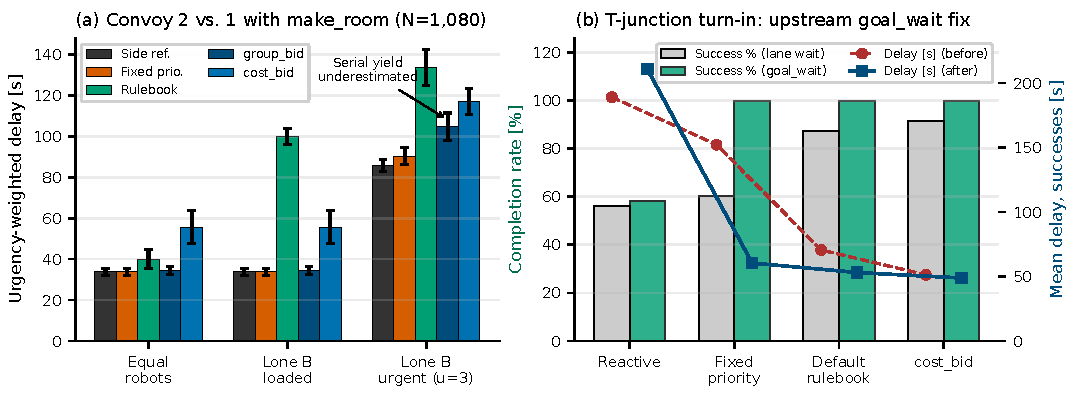
\includegraphics[width=0.74\textwidth]{fig/rq4_topologies.pdf}
\caption{RQ4a---Scaling beyond two-robot straight aisles in 2D. (a) Convoy 2-vs.-1 urgency-weighted delay ($N=1{,}080$) across equal, loaded-$B$, and urgent-$B$ ($u_B=3$) regimes with follower \texttt{make\_room}. (b) Three-robot T-junction turn-in completion rate (bars, left axis) and successful-episode delay (lines, right axis) at $0\%$ loss ($n=48$ per policy) before vs.\ after adding upstream bay waiting (\texttt{goal\_wait}).}
\label{fig:rq4_topo}
\end{figure*}

\smallskip\noindent\emph{Three-Robot T-Junction (384 Episodes):} In the T-junction turn-in study ($A$ bound for branch \texttt{bay1} initially occupied by $S$, while $B$ traverses the main aisle; 48 runs per policy and loss level, Fig.~\ref{fig:rq4_topo}b), holding $A$ in the main corridor deadlocked \texttt{fixed\_priority} in $19/48$ runs ($60.4\%$ completion) at $0\%$ loss. Allowing $A$ to park in upstream \texttt{bay0} via \texttt{goal\_wait} until \texttt{bay1} clears raised completion to $48/48$ ($100\%$) at both $0\%$ and $50\%$ loss for \texttt{fixed\_priority}, \texttt{rules\_default}, and \cb\ (vs.\ $28/48$ for \texttt{reactive}, all failures being deadlocks), with $0\%$-loss delays descending from $60.5\pm 4.7$\,s (\texttt{fixed\_priority}) to $53.1\pm 5.0$\,s (\texttt{rules\_default}) and $48.9\pm 4.0$\,s (\cb, paired advantage $-4.3\pm 2.8$\,s over the rulebook).

\subsection{496-Run Seed-Paired ROS~2 / Gazebo Harmonic Validation}\label{sec:gz}
Because each Gazebo Harmonic episode executes in real time ($\sim 5$\,min wall-clock with launch/reset), we validated transfer on a stratified 460-run main grid spanning every study above (6--10 seeds per condition) plus a 36-run explore-hold/rerun batch, pairing every single Gazebo run with an identical-seed 2D run (Table~\ref{tab:gz} and Fig.~\ref{fig:rq4_gz}). In the 460-run grid, 122 runs executed on the commit immediately preceding explore/obstacle world additions and 338 on the final commit (which altered nothing on default paths); all 36 hold-batch runs executed on the merged hold commit.

\begin{table}[t]\centering
\caption{Seed-paired ROS~2 Jazzy / Gazebo Harmonic transfer summary (460 main validation runs + 36 hold/rerun batch runs).}
\label{tab:gz}
{\footnotesize\setlength{\tabcolsep}{3.0pt}
\begin{tabular}{@{}lrrrrr@{}}\toprule
Scenario / Study Group & Runs & Succ. & Coll. & Same & $\Delta D$ [s] \\\midrule
Single bay, negotiating (\texttt{S1}, S, L) & 70 & 70 & 0 & 70 & $-0.4$ \\
Single bay, \texttt{reactive}               & 10 &  9 & 1 &  5 & $-1.5$ \\
Single bay, forced yielders (O)             & 44 & 44 & 0 & 44 & $-0.5$ \\
Asymmetric urgency / speed (\texttt{S2})    & 36 & 36 & 0 & 36 & $-0.6$ \\
Two bays (\texttt{S4})                      & 30 & 30 & 0 & 30 & $-0.2$ \\
Noisy bids ($\sigma=0.5, 1.0$; \texttt{S7}) & 12 & 12 & 0 &  7 & $+2.2$ \\
Clarke VCG misreports (\texttt{S9})         & 18 & 18 & 0 & 18 & $-0.3$ \\
50\% loss, $0.5$\,s latency (\texttt{S3})   & 18 & 18 & 0 & 18 & $-0.8$ \\
90\% loss, $2.0$\,s latency (\texttt{S8b/c})& 24 & 24 & 0 & 18 & $+4.8$ \\
Convoy 2 vs.\ 1 (\texttt{make\_room})       & 36 & 36 & 0 & 36 & $-0.6$ \\
T-junction (18 exit + 18 turn-in)           & 36 & 36 & 0 & 35 & $-16.8$ \\
Asymmetric static maps                      & 24 & 24 & 0 & 24 & $-0.3$ \\
Physically blocked bay                      & 18 & 18 & 0 & 18 & $-1.2$ \\
Explore (base, $R_{\mathrm{det}}\in\{6,3.5\}$) & 84 & 84 & 0 & 83 & $+0.2$ \\\midrule
\emph{Batch 2:} \texttt{hold\_for\_map}     & 24 & 24 & 0 & 24 & $+10.0$ \\
\emph{Batch 2:} \texttt{det\_3.5} rerun     & 12 & 12 & 0 & 11 & $+3.4$ \\\bottomrule
\end{tabular}}\\[2pt]
{\footnotesize Same: identical first yielder to paired 2D run (fixed by construction on forced runs). $\Delta D$: mean Gazebo minus 2D urgency-weighted delay over paired successes.}
\end{table}

\begin{table*}[t]\centering
\caption{Practitioner policy and protocol selection matrix distilled from $>50{,}000$ 2D and 496 ROS~2 / Gazebo episodes.}
\label{tab:guide}
{\footnotesize\setlength{\tabcolsep}{4.8pt}
\begin{tabular}{@{}>{\raggedright\arraybackslash}p{0.190\textwidth}>{\raggedright\arraybackslash}p{0.20\textwidth}>{\raggedright\arraybackslash}p{0.24\textwidth}>{\raggedright\arraybackslash}p{0.27\textwidth}@{}}\toprule
Deployment Regime & Recommended Policy & Protocol Configuration & Empirical Basis \& Caveats \\\midrule
Homogeneous cooperative fleet; uncertain kinematics ($\sigma \ge 0.5$) & \texttt{rules\_proximity} + $\lambda=0.25$ fairness credit & Periodic \texttt{STATE}/\texttt{BID}; \texttt{share\_map=true}; \texttt{commit} optional & Halves ID-priority excess ($3.1$ vs.\ $6.4$\,s), beats noisy \cb\ above $\sigma=0.5$, reaches $J=0.997$ for $+8.1\%$ delay \\
Heterogeneous cooperative fleet (urgent / loaded / mixed speeds), $\sigma \le 0.25$ & Urgency-weighted \cb & \texttt{share\_map=true} on every \texttt{BID}; \texttt{refuge\_blocked} enabled & $0.04$\,s weighted excess ($98\%$ optimal match vs.\ $27.1$\,s fixed priority); avoids lidar-lag penalty of \texttt{share\_on\_detect} \\
Self-interested / multi-vendor robots sharing aisles & \texttt{clarke} (VCG pivot payment to operator ledger) & Authenticated IDs \& bay sets; audit joint bid scaling & $0.00$\,s unilateral misreport gain ($\le 0.02$\,s realized), but generates $29$--$44\%$ bank surplus and $+4.9$\,s collusion incentive \\
Convoys (2v1) \& branch junctions & \gb\ (equal $u$) or urgency rulebook + \texttt{make\_room}/\texttt{goal\_wait} & Fuse fresh \texttt{STATE} with lidar for occluded junction lanes & \texttt{make\_room} \& \texttt{goal\_wait} restore $100\%$ completion; model \emph{serial} follower clearance when $u_B \gg 1$ \\
Legacy aisle without pull-in bays or off-lane staging queues & \texttt{reservation} (only if staging sits off exit path) & Corridor entry/exit \texttt{STATE} beacons & $100\%$ deadlock-free, but costs $+18.8$\,s excess when mid-aisle bays exist and staging blocks peer exit \\\bottomrule
\end{tabular}}
\end{table*}

\begin{figure*}[t]\centering
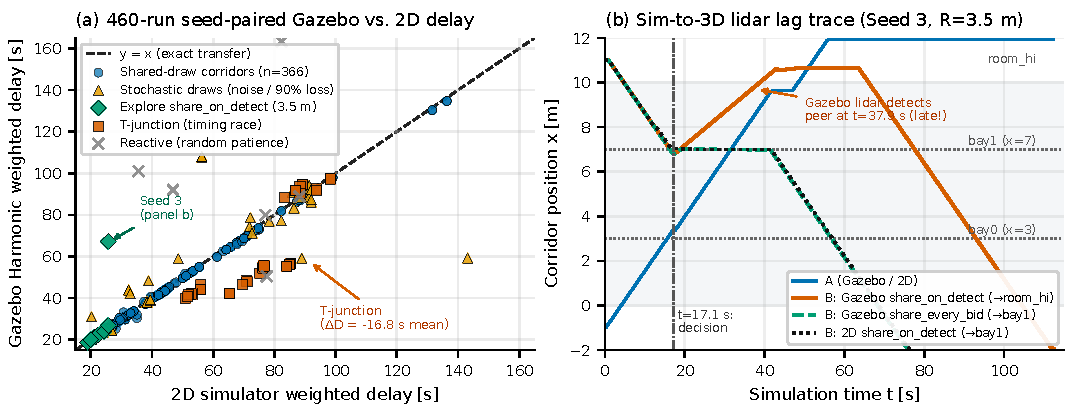
\includegraphics[width=0.74\textwidth]{fig/rq4_gazebo.pdf}
\caption{RQ4b---Sim-to-3D transfer across ROS~2 Jazzy and Gazebo Harmonic. (a) Paired Gazebo vs.\ 2D urgency-weighted delay across the 460-run main grid, showing tight clustering along $y=x$ for all 366 shared-draw corridor runs alongside isolated sim-to-3D divergence in T-junction timing races and $3.5$\,m \texttt{share\_on\_detect}. (b) Empirical spacetime trajectory $x(t)$ on Seed~3 ($R_{\mathrm{det}}=3.5$\,m): wall-filtered Gazebo lidar clustering lags until $t=37.9$\,s, missing the $t=17.1$\,s decision window and sending $B$ to \texttt{room\_hi} instead of \texttt{bay1}.}
\label{fig:rq4_gz}
\end{figure*}

\smallskip\noindent\emph{High-Fidelity Corridor Transfer:} Across all $450$ non-reactive main runs and all $36$ hold-batch runs ($486$ runs total), Gazebo recorded \emph{zero failures and zero collisions} (95\% upper bound $0.85\%$ on the 450 main runs), whereas \texttt{reactive} suffered 1 collision in 10 Gazebo runs. Excluding the 44 forced-yielder baselines, $393$ of $406$ negotiating runs ($96.8\%$) selected the exact same first yielder as their paired 2D episode. Eleven of the 13 yielder differences stem from intentionally unshared stochastic realizations: 5 noisy-bid runs (where log-normal noise hashes decision timestamp \texttt{round(t,1)}, which shifts slightly under ROS~2 scheduling) and 6 independent $90\%$-loss runs (including safeguarding all-on vs.\ all-off at $0.26$\,m/s). Across all 366 shared-draw corridor runs (blue circles in Fig.~\ref{fig:rq4_gz}a), Gazebo excess delays against Gazebo's own forced-yielder reference matched 2D within $\le 1.0$\,s for every policy (\texttt{fixed\_priority} $7.5$ vs.\ $7.6$\,s; \texttt{reservation} $15.2$ vs.\ $15.2$\,s; \texttt{learned} $5.1$ vs.\ $5.3$\,s; \cb\ and \texttt{clarke} $0.0$\,s in both).

\smallskip\noindent\emph{Three Concrete Sim-to-3D Gaps:} Crucially, Gazebo physics exposed three structural boundaries invisible to 2D unicycle sweeps:
\begin{enumerate}
\item \emph{Lidar peer-clustering latency (\texttt{explore} \& \texttt{hold\_for\_map}):} Whereas \texttt{sim2d} registers peers instantaneously at $3.4$\,m inside the $3.5$\,m lidar circle, Gazebo's wall-filtered \texttt{LaserScan} clustering (\texttt{cluster\_dist} $0.35$\,m matched within $2R_{\mathrm{sw}}=0.50$\,m of peer \texttt{STATE}) first registers an oncoming Waffle at $2.3$--$2.6$\,m separation on average. Consequently, at $R_{\mathrm{det}}=3.5$\,m, \texttt{share\_on\_detect} delivered $0/6$ maps before decision in Gazebo vs.\ $6/6$ in 2D (Fig.~\ref{fig:rq4_gz}b), inflating \texttt{fixed\_priority} delay by $+7.0$\,s over Gazebo full-map ($+6.8$\,s over 2D). Enabling \texttt{hold\_for\_map} (24 Gazebo runs) restored near-bay selection (\texttt{bay1}) in $24/24$ runs, but peer detection occurred even closer ($1.10$--$1.18$\,m, waiting $4.7$\,s at $3.5$\,m and $9.5$\,s at $6.0$\,m after conflict onset), costing $+10.0$--$10.1$\,s over Gazebo full-map; by detection time, $A$ ($6/6$) and $B$ ($5/6$) had already self-sensed both bays, meaning holding worked in 3D by delaying decisions rather than via map exchange. Piggybacking maps on every \texttt{BID} avoids this gap entirely.
\item \emph{Branch-wall lidar occlusion:} Pre-final Gazebo T-junction runs revealed that the $2.0$\,m side-branch walls physically occlude a parked branch robot's lidar view of the main aisle (and that 2D lacked wall checks on room goals), motivating the fusion of fresh \texttt{STATE} positions into lane-clearance checks; accordingly, T-junction Gazebo runs serve as a post-fix verification rather than an independent blind test.
\item \emph{Three-robot T-junction timing sensitivity ($\Delta D=-16.8$\,s):} Across all 36 T-junction runs, Gazebo finished $605.3$\,s faster cumulatively than 2D ($-260.0$\,s across 18 exit runs; $-345.4$\,s across 18 turn-in runs). Event traces pinpoint the exit discrepancy (\cb\ $-264.7$\,s, \texttt{fixed\_priority} $+18.6$\,s, rulebook $-14.0$\,s) to a $\sim 20$\,s release-timing race: in Gazebo, branch robot~$S$ exits \texttt{bay1} slightly earlier relative to $A$'s parked window under \cb\ and slips past without triggering the second head-on conflict (or occasional $60$\,s proceed-timeout stall) seen in 2D, whereas under \texttt{fixed\_priority}/rulebook $S$ meets $A$ holding in-lane and yields a second time ($4/4$ and $3/4$ runs). The larger turn-in offset ($9.5$--$28.9$\,s lower delay per run; $0.4$--$6.4$\,s shorter makespan) remains an open sim-to-3D timing gap, so quantitative T-junction delays cannot be inferred from 2D alone.
\end{enumerate}

\section{Discussion, Practitioner Guidelines, and Limitations}\label{sec:disc}

\subsection{Synthesis and Fleet Engineering Selection Matrix}
Stepping back across RQ1--RQ4, head-on single-lane coordination separates cleanly into a \emph{decision mechanism} choice governed by fleet heterogeneity, cost-model accuracy, and ownership incentives, and a \emph{protocol execution} layer governed by radio reliability, map consistency, and multi-robot geometry. Table~\ref{tab:guide} distills our quantitative findings into an actionable selection matrix for AMR system architects.

Three cross-cutting lessons stand out. First, \emph{broadcasting intent with piggybacked refuge IDs dominates complex handshakes}: periodic \texttt{BID} snapshots carrying known/blocked bays eliminate static and online map penalties at zero delay cost, whereas explicit \texttt{commit} handshakes add $3$--$4$\,s under extreme loss without reducing collisions or deadlocks, and lidar-gated \texttt{share\_on\_detect} breaks in 3D Gazebo due to peer-clustering lag. Second, \emph{cost-model fidelity and objective alignment bound optimization gains}: optimizing unweighted delay under heterogeneous urgency wastes twice as much weighted time ($7.0$\,s) as a 6-line rulebook ($3.5$\,s), and scalar bid noise of $\sigma=0.5$ erases \cb's advantage entirely. Third, \emph{pairwise additive approximations break before physics does}: straight-corridor 2D excess delays transfer within $1.0$\,s to Gazebo, whereas multi-robot serial convoy clearances and T-junction stem-release races require explicit multi-agent timeline modeling and 3D physics-in-the-loop testing.

\subsection{Limitations and Future Scope}
Our study has explicit boundaries that frame future work:
\begin{itemize}
\item \emph{Simulation-only evaluation and ground-truth pose:} All results come from 2D and Gazebo Harmonic simulation (6--10 non-deterministic runs per Gazebo cell), with Gazebo nodes reading ground-truth pose so AMCL/SLAM localization drift, wheel slip, and physical TurtleBot3 hardware transients remain untested.
\item \emph{Shared kinematic structure and non-bid strategic attacks:} \cb\ and \texttt{clarke} use the simulator's true speed limits and refuge coordinates; structural model mismatches, strategic bay-omission attacks, \texttt{commit}-ID spoofing, budget-redistribution schemes, and individual rationality are not evaluated.
\item \emph{Local baseline and liveness theory:} Only centerline \texttt{reactive} backoff was run without communication (not continuous ORCA, RVO, or CBF controllers), the protocol lacks a formal termination bound for transient mutual yields ($14$--$24\%$ under extreme loss), and the best forced yielder is a decision-level rather than globally optimal trajectory reference.
\item \emph{Topological approximations and deliberation latency:} The T-junction models a branch as a $2$\,m-deep bay (with an unexplained $-345.4$\,s turn-in Gazebo offset), \texttt{explore} performs geometric range discovery rather than SLAM, map-mismatch/obstacle cells use 10 seeds, and \texttt{learned} is a centralized tabular bandit rather than deep MARL. Finally, all policies studied here compute decisions in sub-millisecond CPU time; foundation-model and LLM negotiators~\cite{marlin2024,gamechat2025,garg2024llm} introduce multi-second inference latencies while robots remain in motion as well as anti-coordination failure modes that require dedicated asynchronous protocol mechanisms and separate empirical investigation.
\end{itemize}

\section{Conclusion}\label{sec:conc}
We introduced an open dual-simulator benchmark for head-on narrow-corridor AMR encounters with discrete pull-in bays, executing identical 20\,Hz agent code across more than 50,000 2D episodes and 496 seed-paired ROS~2 Jazzy / Gazebo Harmonic runs. Negotiating policies eliminate the $6.2\%$ deadlock rate and $\ge 3.6\times$ delay penalty of zero-communication reactive backoff. Kinematic cost bidding matches the hindsight yielder reference across symmetric corridors and cuts asymmetric weighted excess delay to $0.04$\,s, reaching parity with a closest-refuge rulebook at log-normal bid error $\sigma=0.5$. Clarke-pivot VCG payments eliminate unilateral scaled-misreport gains at the cost of a $29$--$44\%$ budget surplus and joint-collusion exposure, while a lightweight cumulative-delay credit ($\lambda=0.25$) achieves $0.997$ Jain fairness for $8.1\%$ extra delay. Periodic snapshot broadcast with piggybacked bay lists sustains zero collisions through 99\% packet loss and partial maps, and transfers $96.8\%$ of yield decisions and $\le 1.0$\,s straight-corridor excess delays to 3D Gazebo while exposing concrete lidar-clustering and junction-timing transfer boundaries. All source code, worlds, scripts, and per-episode records are publicly released at \url{[ANONYMIZED-URL]}.

\patchcmd{\thebibliography}{\footnotesize}{\footnotesize\setlength{\itemsep}{0pt}\setlength{\parskip}{0pt}\linespread{0.88}\selectfont}{}{}
\bibliographystyle{IEEEtran}
\bibliography{refs}

\end{document}
